\chapter{脑膜刺激征}

由于软脑膜本身的炎征或受刺激时出现一系列提示脑膜受损的病征,如头痛、呕吐、颈肌强硬、克匿格(Kernig)征与布(Brudzinski)氏征阳性、皮肤感觉过敏、对听觉和视觉刺激过敏等,称为脑膜刺激征。头痛是最常见且早期出现的症状,通常为弥漫性,但枕部和额部特别显著。头痛的发生是由于分布在脑膜的三叉神经与迷走神经感觉性终末器受炎症性及机械性刺激(颅内压过高)所致。脑膜刺激征一方面由脑膜本身病变所引起,另外也可由于颅内其他病变如颅内压增高、脑炎、脑水肿等所引起。

有报告坐位低头试验和贴膝试验对早期发现脑膜刺激征甚有帮助,当出现早期脑膜炎和轻度脑膜刺激反应、而常规体格检查尚属阴性时,可较早地出现阳性。如两种检查为阳性,即可认为有早期脑膜刺激征的存在,而作为腰椎穿刺检查脑脊液的指征,可达到各种脑膜炎早期发现、早期治疗的目的。

\section{(1)坐位低头试验:}

患者取坐位,两下肢伸直,使下肢与躯干呈直角,嘱患者低头至下颌触及前胸为正常(阴性);如低头受限制,下颌不能触及前胸或发生疼痛则为阳性。

\section{(2)贴膝试验:}

患者取坐位,两下肢于髋、膝关节随意屈曲,嘱患者以口贴膝或以下颌触膝,能贴及或触及者为正常(阴性)。如不能者则为阳性。

必须指出,婴幼儿、老年人、体弱者患脑膜炎时,不一定有典型的脑膜刺激征出现,可疑时应及时作脑脊液检查,以免漏诊或误诊。

此外,判断脑膜刺激征时应注意下列几点:

(1)脑膜炎时脑膜刺激征很显著,颈强直更突出,甚至出现角弓反张。

(2)颅内压增高程度与脑膜刺激征平行,脑疝时往往颈强直明显而克匿格征与布氏征不突出。

(3)蛛网膜下腔出血时首发症状常是头痛,颈强直有时立即出现,有时经数小时或48小时才出现。

(4)婴幼儿因颅骨骨缝未闭合故脑膜刺激征不典型,此时应注意囟门变化,囟门膨隆可作为参考。

(5)脑膜刺激征在深昏迷时消失。

\section{【脑膜刺激征的疾病分类】}

\begin{table}[htbp]
\centering
\caption{引起脑膜刺激征的疾病分类}
\label{tab50-1}
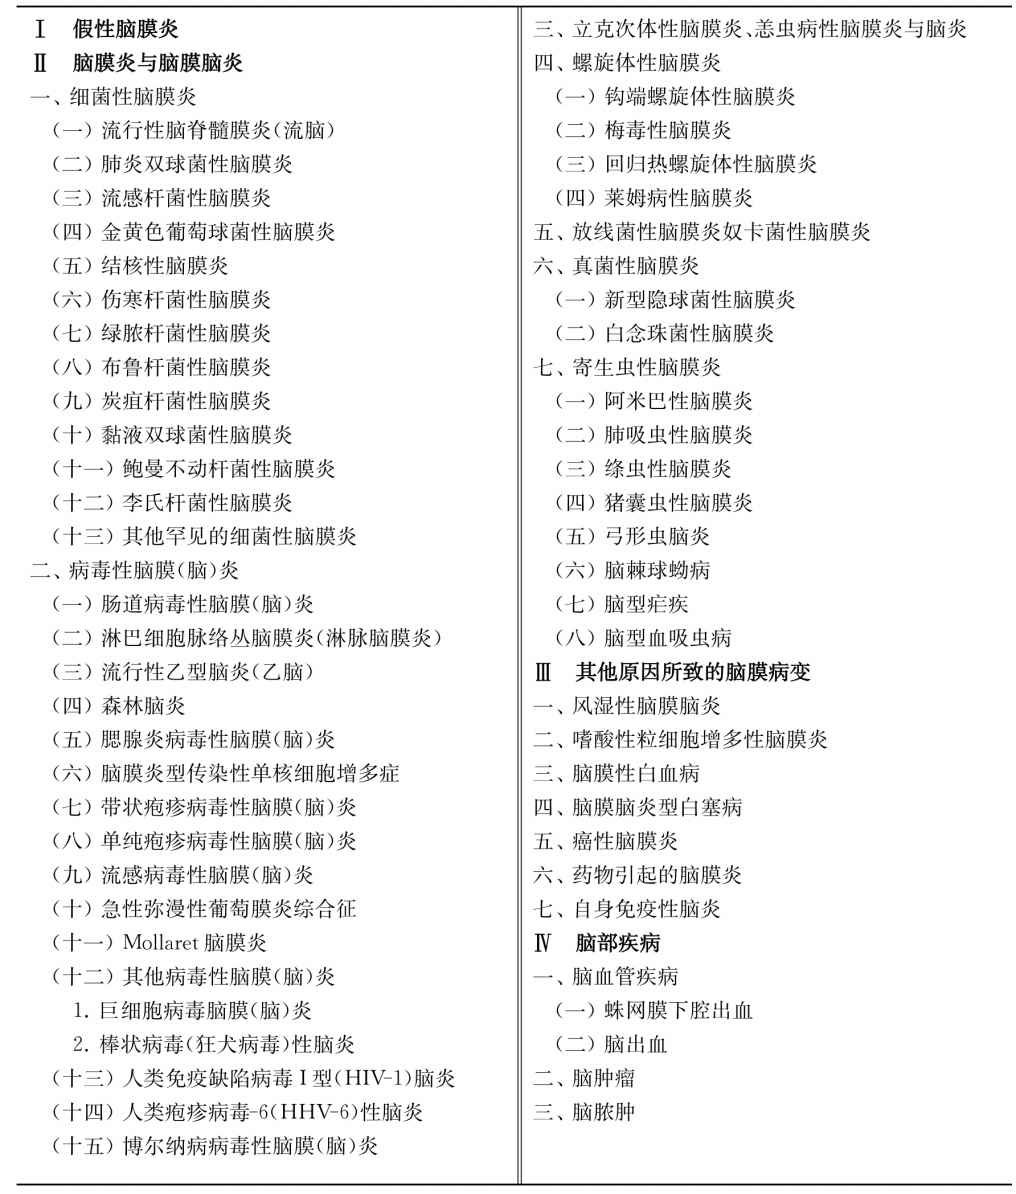
\includegraphics[width=5.9375in,height=6.97917in]{./images/Image00311.jpg}
\end{table}

\protect\hypertarget{text00383.html}{}{}

\section{165 假性脑膜炎}

假性脑膜炎(meningismus)以脑膜刺激征为临床特征,偶尔伴抽搐及昏迷。假性脑膜炎常出现在急性发热疾病起病时,以婴幼儿多见。肺炎、扁桃体炎、猩红热与肾盂肾炎可引起假性脑膜炎是众所周知的。脑脊液检查压力增加,而细胞数一般正常(偶尔可稍增)、糖量正常、蛋白量与氯化物通常不高、病原体检查阴性。该征症状与脑脊液的改变可能系血液与脑脊液之间的平衡失调所致。有文献认为,在急性感染起病时,血液迅速被稀释,形成相对的低张,液体迅速经由脉络丛滤入脑脊液中,致脑脊液压力增加。假性脑膜炎的诊断主要依靠脑脊液检查。经积极的治疗之后,脑膜刺激症状一般于数天之内消失。假性脑膜炎也可见于败血症、伤寒与副伤寒、中毒型菌痢、斑疹伤寒、恙虫病、流行性感冒、钩端螺旋体病、急性疟疾等急性感染过程中。

\protect\hypertarget{text00384.html}{}{}

\section{166 脑膜炎与脑膜脑炎}

按病因学不同脑膜炎(脑脊髓膜炎)基本上可区分为细菌性、病毒性、螺旋体性、真菌性与寄生虫性五大类。按脑脊液的性质而将脑膜炎划分为化脓性、浆液性与出血性等类型。

化脓性脑膜炎的脑脊液特征是压力升高,微浑、毛玻璃样乃至米汤样,细胞数>1000×
10\textsuperscript{6}
/L,分类以中性分叶核粒细胞占优势,球蛋白显著增多,糖与氯化物明显减少,可通过涂片染色检查或培养发现病原菌。化脓性脑膜炎又可进一步区分为原发性与继发性两类。原发性化脓性脑膜炎主要见于流行性脑膜炎(流脑),也可见于流感杆菌性脑膜炎或新生儿期的混合细菌性脑膜炎。继发性化脓性脑膜炎则通常继发于大叶性肺炎、化脓性中耳炎、鼻窦炎、乳突炎、颅部外伤合并感染、败血症、细菌性心内膜炎等。

浆液性脑膜炎的病因众多,脑脊液的特征是压力升高或正常,透明澄清、微浑或毛玻璃样,细胞数通常在1000×10\textsuperscript{6}
/L以下,分类以淋巴细胞为主(早期可能中性分叶核粒细胞稍占优势),球蛋白增多,糖与氯化物大都正常(结核菌及真菌感染例外),可通过涂片染色检查、细菌培养、病毒分离、免疫学试验及动物接种等确诊。浆液性脑膜炎最常由病毒所致,但结核菌、螺旋体、真菌、寄生虫等脑膜感染,脑脓肿、化脓性中耳炎、乳突炎、鼻窦炎等灶性感染所致的反应性脑膜炎,以及未经充分治疗的化脓性脑膜炎等也可表现为浆液性。

出血性脑膜炎的脑脊液特征是压力升高,呈血性浑浊,内含大量红细胞,白细胞也增多,白细胞∶红细胞>1∶500(此点有助于鉴别单纯性蛛网膜下腔出血),球蛋白增多,糖与氯化物正常或减少(因病因不同而异),可通过相应的病原学与免疫学检查而确立诊断。

有报道肿瘤坏死因子α(TNFα)测定有助于细菌性脑膜炎与病毒性脑膜炎的鉴别。研究结果表明脑脊液中TNFα含量的高低依次为:化脓性脑膜炎急性期(33.92±1.51)>结核性脑膜炎(18.46±1.62)>化脓性脑膜炎恢复期(10.54±1.90)>病毒性脑炎(8.18±3.30)。这种情况有助于细菌性脑膜炎与病毒性脑膜炎的鉴别。

\subsection{一、细菌性脑膜炎}

\subsubsection{(一)流行性脑膜炎(流脑)}

流脑的主要临床特征是高热、脑膜刺激征与皮肤黏膜出血。凡在流脑容易发生的冬、春二季,患者(尤其是儿童或青少年)突然发病而兼有上述表现,大致可诊断为流脑。皮肤出血点压片染色镜检可发现脑膜炎双球菌,阳性率高达87.4\%,方法简便易行,对早期确诊流脑提供可靠依据。

涂片检查法:首先选择较典型的出血点,消毒皮肤后,用注射针头沿瘀点边缘向内作浅斜穿刺,用手指从旁边轻挤出淤血,以洁净玻片直接印涂数片,待其自然干燥,用碱性亚甲蓝溶液染色,水洗干燥后镜检。如菌形态不典型,取另一涂片作革兰氏染色对照。

流脑通常以寒战、高热急骤起病。脑膜刺激征象往往在24小时内出现。此时高热持续,头痛剧烈,颈项强硬而痛,呕吐频繁,每呈喷射性。患者眼结膜充血、怕光、烦躁不安、神志不清,常发生谵妄、抽搐与昏迷。皮肤黏膜出血见于大多数病例,最早出现在眼结膜及口腔黏膜,对早期诊断甚有帮助。皮肤出血点逐渐增多提示有发生休克的可能。唇疱疹虽仅见于部分病例,但唇疱疹(病期第3~6天出现)对流脑与结核性脑膜炎和其他化脓性脑膜炎的鉴别颇有意义。

典型流脑的诊断不一定需作脑脊液检查,但非典型性病例与散发性病例常需借助腰椎穿刺脑脊液检查以明确诊断。流脑的脑脊液呈化脓性炎症改变,涂片染色镜检可发现肾形的革兰氏阴性双球菌(红色),阳性率达61\%~74\%,对确诊有重要价值。如同时作双份脑脊液涂片检查可增加阳性机会。必须指出,早期病例尤其是暴发型脑膜炎双球菌败血症早期脑脊液往往正常,因此这时脑脊液无异常绝不能轻易除外流脑。

有的结核性脑膜炎患者起病较急,在流脑流行期间每易与流脑相混淆;反之,流脑患者可因治疗不当致病程迁延而误诊为结核性脑膜炎。蛛网膜下腔出血偶尔也可误诊为流脑,而个别流脑患者的脑脊液又可呈现出血性炎症改变。此时,详细追问病史(发热在先者为流脑,反之则为蛛网膜下腔出血)、计算脑脊液红、白细胞比例与涂片染色找病原菌,以及糖定量检查,对两者的鉴别有重要意义。此外,在流脑流行期间,如发现患者的脑脊液呈化脓性炎症改变,虽未能找到脑膜炎双球菌,而临床上可除外其他原因所致的化脓性脑膜炎者,流脑的诊断也可成立。

\subsubsection{(二)肺炎双球菌性脑膜炎}

肺炎双球菌性脑膜炎以婴儿及老年人多见,可发生于大叶性肺炎兼有败血症的过程中,也可直接由耳、鼻、咽部化脓性(如中耳炎、乳突炎、鼻窦炎)蔓延而来,或继发于颅部外伤骨折后。少数病例可能以上呼吸道或其他创口为侵入途径,而无明显的感染来源,此即所谓原发性病例。如此病例继发于大叶性肺炎,大都发生于肺炎病程第5~6天以后;由于原发病的病情较重,又可出现假性脑膜炎症状,脑膜炎征象每被掩蔽,其发病日期颇难明确。如原发感染灶未根治,肺炎双球菌性脑膜炎可再发。

临床表现为急性化脓性脑膜炎的征象,以发病急骤与预后险恶为特征,且可能复发。确诊需依靠脑脊液检查。国内报告的121例中血培养仅25\%阳性,但脑脊液呈脓样混浊,及时涂片染色检查阳性率达86.7\%,甚有早期诊断意义。值得注意的是,婴幼儿或老年人患暴发型肺炎双球菌脑膜炎时,脑脊液细胞数可正常,但沉淀后涂片染色镜检往往发现大量肺炎双球菌。临床上凡患者有大叶性肺炎、头部感染或颅部外伤骨折史而发热不退,并出现脑膜刺激征时,需考虑并发肺炎双球菌性脑膜炎的可能性。

\subsubsection{(三)流感杆菌性脑膜炎}

流感杆菌性脑膜炎主要侵犯1岁以下婴儿,少见于4岁以上儿童,成人则罕见。国内报告的一组病例中发病率以10月份最高,其次为9月,说明发病与呼吸道感染有较密切的关系。临床上主要表现为急性化脓性脑膜炎病象,但发病开始时往往先有上呼吸道炎症状,且病程中出现皮肤黏膜瘀点者甚罕见。脑脊液检查符合化脓性炎症改变,涂片染色容易检出革兰氏阴性流感杆菌,阳性率达81.2\%,对早期诊断有重要价值。脑脊液培养及血培养有助于确诊。凡患儿有嗜睡、易于激动、幻觉或突然尖声哭叫等可疑脑症状时,需考虑此病的可能性,并及时作脑脊液检查以明确诊断。

有的早期病例尤其是未经充分治疗的患者,脑脊液检查呈无菌性(浆液性)炎症改变,每易误诊为结核性脑膜炎,需注意鉴别之。

\subsubsection{(四)金黄色葡萄球菌性脑膜炎}

此病是化脓性脑膜炎中严重的一种,较易侵犯儿童,尤以2岁以下婴幼儿为多见。传染途径有三:①由远处病灶经血行播散;②由原发感染灶直接蔓延,例如中耳炎、乳突炎、鼻窦炎、面部蜂窝织炎、脊椎或颅骨骨髓炎、硬脊膜外脓肿或脑脓肿等;③由颅部骨折性外伤、神经外科手术或诊断性穿刺直接感染。一般认为前两者为主要侵入途径。

起病缓急不一,部分病例起病较缓。据国内报告的45例中,临床表现有两点较为特别:①颈项强硬的发生率与强度均较一般脑膜炎高;②各种类型皮疹的出现,包括瘀点、瘀斑、荨麻疹、小脓疱等。脑脊液外观可自微浑、毛玻璃样乃至凝成奶糕样。蛋白含量一般较高,但部分病例细胞数低于1000×10\textsuperscript{6}
/L,此种情况值得注意,因单凭细胞计数可被误诊为乙型脑炎、结核性脑膜炎、无菌性脑膜炎等。半数以上脑脊液培养阳性,血培养与脑脊液涂片检查也有助于诊断。

\subsubsection{(五)结核性脑膜炎}

结核性脑膜炎(TBM)多见于儿童,但成人也非少见。发病年龄与一般结核病相同。患者多有肺、骨、胸膜或淋巴结结核病史。发病多徐渐,也可相当急骤。妊娠、分娩是女性患者的主要诱因。患者以全身不适、畏寒、发热、头晕、头痛、全身酸痛等症状起病。发热与头痛是最常见于最早出现的症状。有的患者自觉无发热,但测温时发现体温升高。早期病例常被误诊为感冒;如患者消化系统症状明显而兼有表情淡漠,每易与伤寒相混淆。各项体征以颈抵抗出现最早,故对此病有早期诊断意义。此时脑脊液一般已有改变,压力大多升高,澄清、无色或微浑呈毛玻璃样,静置后往往有薄膜形成,细胞增多一般在(50~500)×
10\textsuperscript{6}
/L之间,分类以淋巴细胞占优势(早期可能以中性分叶核粒细胞稍占优势),糖与氯化物减少。透明澄清的脑脊液,而糖量(低于35mg\%)与氯化物(低于700mg\%)一致下降,对结核性脑膜炎的诊断有重要意义(需除外真菌性脑膜炎),并可据此与病毒性脑膜(脑)炎相鉴别。脑脊液色氨酸与利文生试验的阳性率颇高,对诊断有一定帮助。脑脊液涂片染色检查可发现结核杆菌,从薄膜中较易检出,阳性率为37.9\%~64.4\%不等,有确诊价值。如脑脊液中结核杆菌虽为阴性,但始终未发现其他细菌或真菌,而抗结核治疗效果明显者,也大致可确定此病的临床诊断。眼底检查12.7\%~80\%的病例可发现视网膜结节,于视盘附近单个或成组出现,初始为黄色,边界不清,随病程进展周边可出现色素沉着。此种结节的出现对结核性脑膜炎的诊断有重要意义。CT、MR等影像学检查不能确诊结核性脑膜炎,但在临床疑诊时,某些特征性改变则有一定的参考意义。

TBM的诊断除临床症状、体征外,脑脊液(CSF)的实验室检测极其重要。近年来有关CSF检测项目在TBM诊断中的研究已取得了长足发展,其中CSF常规结合PCR、抗原抗体检测对TBM的诊断、病情评估具有一定价值。但一些检查指标的特异性、灵敏度尚不令人满意。主要包括下列几个方面:

\paragraph{1.细胞学检查}

TBM的CSF细胞学改变具有一定的规律性特征,其特点是以中性粒细胞为主伴一定数量的免疫活性细胞(小淋巴细胞、淋巴样细胞和浆细胞)和单核吞噬细胞的混合细胞反应,亦可见到嗜酸性粒细胞。尽管持续抗结核治疗,CSF细胞学的混合细胞反应可持续4周,预后较好者中性粒细胞减少,免疫活性细胞相对增高(Rhem交叉现象)。CSF中淋巴样细胞和浆细胞的阳性率明显增高是TBM早期的一个重要特征,若能结合生化检查和临床表现,可为TBM的早期诊断提供有力依据。

\paragraph{2.病原学检测}

CSF分离抗酸杆菌仍然是确诊TBM最直接可靠的方法,反复送检可提高阳性率。

\subparagraph{(1)直接涂片法:}

自从1882年以来,涂片抗酸染色一直是检查结核杆菌的重要方法。该方法最为简单经济,但敏感性、特异性较差,在一般离心沉渣中难以收集到结核杆菌,国内外学者报告涂片阳性率约为10\%。为提高涂片的阳性率,一些学者提出加大离心转速、延长离心时间,用静止CSF标本析出的纤维蛋白膜染色镜检等方法。采用漂浮浓集法和离心浓集法,可使涂片阳性率达到92.19\%和62.15\%;取CSF静置24小时后形成薄膜,涂片抗酸染色镜检阳性率可达到91.0\%。

\subparagraph{(2)结核杆菌培养法:}

培养法的优点是直观,可作进一步鉴别、药敏和毒力检测。但结核杆菌生长缓慢,培养需4~8周,且阳性率在20\%~30\%。有研究者用改良Levinson析出法对64例TBM和54例可疑诊断TBM标本进行检测,阳性率分别为93.7\%和85.5\%,而采用Levinson法的阳性率分别为79.7\%和72.2\%,结合CSF分析可确诊89\%的TBM,显示了一定的优越性。

\subparagraph{(3)聚合酶链反应(PCR)检测结核分枝杆菌DNA:}

PCR技术自1985年Saiki建立该方法以来发展很快,1990年以来国内各大医院已将其用于临床,在TBM的早期诊断和鉴别诊断中具有参考价值,其敏感性及特异性优于以往病原学检查常用的抗酸染色及结核菌培养。本方法目前存在的最大问题是易出现假阳性结果。

\paragraph{3.生化分析}

\subparagraph{(1)乳酸:}

许多学者对CSF乳酸(CSF2LA)测定的评价较高,认为其是鉴别细菌性和病毒性脑膜炎的重要方法。CSF2LA含量测定有气液色谱法和酶法两种,以3~125mmol/L为正常值界限,研究证实TBM的CSF2LA含量显著增高。

\subparagraph{(2)氨基酸:}

Qureshi等的研究发现亚硝酸盐和其前体精氨酸、高半胱氨酸在TBM显著增高,苯丙氨酸增加和氨基乙磺酸及维生素B\textsubscript{12}
降低也仅在TBM发现。在临床工作中,我们可根据这些重要生化指标的变化设计治疗方案。

\subparagraph{(3)酶活性测定}

1)腺苷脱氨酶(ADA):ADA是与机体细胞免疫有密切关系的核酸代谢酶,与T淋巴细胞增殖、分化密切相关。CSF2ADA活性在TBM患者明显升高,阳性率可达80\%~90\%,可作为TBM的早期诊断指标之一。

2)乳酸脱氢酶(LDH):LDH在体内分布广泛,脑组织中含量较高,多种疾病均可引起升高,是反映疾病的敏感指标,相应的特异性很低。然而LDH同工酶测定可显著地改善其特异性,在TBM的诊断中非常有用。Kamat等发现LDH及其同工酶可作为各型脑(膜)炎的鉴别诊断工具:TBM患者LDH4活性增高;化脓性脑膜炎是LDH3活性增高;病毒性脑炎则是LDH2和LDH1活性增高。

3)其他:CSF腺苷酸激酶、谷氨酸脱羟酶(GAD)、谷氨酸脱氢酶(GLDH)的活性水平在TBM时显著升高。

\paragraph{4.免疫学检测}

\subparagraph{(1)细胞免疫检测:}

研究发现,CSF中活性B细胞(ABL)在发病早期的出现率较高,阳性率为65.5\%,特异抗体稍后出现,CSF的细胞数与淋巴细胞中ABL的百分率在病程中存在正相关关系。

\subparagraph{(2)体液免疫检测:}

在TBM时CSF2Ig系列指标明显升高,中枢神经系统24小时鞘内IgG合成率(IgG2syn)明显增高,且与病情的严重程度有关,可以作为TBM患者病情严重程度、疗效及预后判断的重要指标。

\subparagraph{(3)结核分枝杆菌硬脂酸检测:}

结核分枝杆菌硬脂酸(102甲基十八烷酸)(TSA)是结核杆菌菌体中的特有成分,用气相色谱法检测有很高的敏感性和特异性。

\subparagraph{(4)结核抗原检测+抗结核抗体检测:}

ELISA、RIA或LPA法检测CSF中的结核抗原,已成功地用于TBM的早期诊断,而用阿拉伯糖甘露糖脂(LAM,分枝杆菌细胞壁外表面特有的一种成分)抗原检测特异性IgG抗体(LAM2IgG),对快速诊断TBM也有较高的应用价值。由于ELISA法检测结核抗原和抗结核抗体本身就存在5\%左右的假阳性或假阴性可能,因此应尽可能同时进行抗原抗体检测。

\paragraph{5.细胞因子检测}

肿瘤坏死因子(TNFα)、可溶性白介素2受体(sIL22R)、基质金属蛋白酶谱(MMPs)及粒细胞集落刺激因子(G2CSF),均可作为TBM的辅助诊断。

\subsubsection{(六)伤寒杆菌性脑膜炎}

伤寒杆菌性脑膜炎罕见,国内仅有少数病例报告。此病可发生于伤寒病程的任何时候,但以病程第一周内较多见。临床上病情较重,常有意识障碍或昏迷。脑脊液呈化脓性炎症改变,培养可发现伤寒杆菌。此病每易与结核性脑膜炎相混淆,需注意鉴别。

\subsubsection{(七)绿脓杆菌性脑膜炎}

绿脓杆菌性脑膜炎少见,国内仅有少数病例报告。本病多见于颅脑外伤病例,也可因诊断性或治疗性腰椎穿刺过程中消毒不严污染所致。临床上除表现为急性化脓性脑膜炎征象与病程进展较缓外,最特征性的改变是脑脊液呈黄绿色,此点为其他化脓性脑膜炎所没有,具有重要的诊断价值。脑脊液的颜色深度往往与症状的轻重、细胞数的多少以及培养阳性率的高低呈正比。必须指出,有的病例脑脊液非呈黄绿色,故脑脊液无黄绿色改变不能轻易除外绿脓杆菌性脑膜炎,有怀疑时需及时作脑脊液培养以明确诊断。

\subsubsection{(八)布鲁杆菌性脑膜炎}

布鲁杆菌性脑膜炎少见,国内仅有少数病例报告。波状热常并发中枢神经系统症状,并发脑膜炎时则出现脑膜刺激征。如高度怀疑为脑膜炎,则需进行腰椎穿刺作脑脊液检查。脑脊液压力多见增高,外观澄清或轻度浑浊,偶尔可呈脓样浑浊,细胞数增多,细胞分类及大部分为淋巴细胞,蛋白量增高,每在100mg\%以上,糖量减少,氯化物正常或稍低,培养或动物接种可发现布鲁杆菌。脑脊液布鲁杆菌凝集反应及补体结合试验多呈阳性,但有些无中枢神经系统并发症的波状热患者也可呈阳性反应。本病与其他原因脑膜炎的鉴别主要根据流行病学史、临床表现、脑脊液检查以及有关的细菌血清学检查。

\subsubsection{(九)炭疽杆菌性脑膜炎}

炭疽杆菌侵及中枢神经系统时引起脑膜刺激征及脑膜出血性炎症。炭疽杆菌性脑膜炎少见,国内只有少数病例报告。脑脊液检查对诊断有决定性意义。脑脊液呈血性,压力增高,蛋白量与细胞数显著增多,糖显著减少或阴性,涂片与培养均可发现大量革兰氏染色阳性大杆菌,两端呈方形,互相连接成链状。炭疽杆菌性脑膜炎的预后险恶,临床医生需倍加警惕。此病的诊断线索为与病畜或其皮毛接触史,或原发皮肤炭疽感染灶的发现;如接触史不明,诊断常被忽视。此病需与蛛网膜下腔出血或其他原因所致的出血性脑膜炎相鉴别。

\subsubsection{(十)黏液双球菌性脑膜炎}

国内发现一些革兰氏阴性球、杆菌------硝酸盐还原试验阴性杆菌(B-anitratum)与mima菌感染。此类细菌临床上可引起脑膜炎合并败血症、肺炎合并败血症、亚急性细菌性心内膜炎、败血症、上呼吸道感染等。此型脑膜炎为散发性,临床表现类似流行性脑膜炎,严重时甚至可引起华-弗综合征。脑脊液及皮疹刮出物涂片染色可检出此菌,血培养或皮疹刮出物培养也可获阳性结果。此菌与脑膜炎双球菌在形态上很相似,但两者的药物敏感性不同,需注意区别。国内曾有报告烧伤后并发此型脑膜炎,并称为黏液双球菌性脑膜炎。

\subsubsection{(十一)鲍曼不动杆菌性脑膜炎}

鲍曼不动杆菌是一种专性需氧、在光学显微镜下形态多为球形或成双排列的革兰氏阴性球杆菌,广泛存在于外界环境中,是人类和动物皮肤、呼吸道、胃肠道的正常菌群,也是医源性脑膜炎、中耳炎、败血症的条件致病菌。该菌所致医院感染逐年增加,特别在与脑外科手术或脑室引流相关的脑膜炎中扮演重要角色;同时,随着耐药菌株的出现,术后脑膜炎的治疗越发棘手,病死率高。

鲍曼不动杆菌性脑膜炎的临床表现为发热及不同水平的意识障碍,这是最常见的症状,之后出现头痛、抽搐、恶心、呕吐症状。最常见的是脑膜炎刺激征及颅脑手术处的局部膨胀。

CSF检查提示以中性淋巴细胞为主的细胞增多,蛋白水平增高及低葡萄糖。其诊断标准如下:①CSF培养出鲍曼不动杆菌;②非其他原因导致的下列至少一项症状:发热(38℃),头痛,脑膜刺激症状,脑神经功能障碍或刺激症状;③CSF至少有以下一项改变:白细胞增高,蛋白增高和(或)葡萄糖低;④患者获得性感染的时间于住院72小时后和(或)侵入性检查后。葡萄糖、蛋白及细胞计数正常的CSF培养阳性,无临床症状的患者为隐性感染。

\subsubsection{(十二)李氏杆菌性脑膜炎}

李氏杆菌病十分罕见。该病可以散发或者呈食源性暴发出现。与其他的食源性微生物不同,李氏杆菌可以在冷藏的食物中自行复制。孕妇、新生儿、免疫缺陷者及老年人均能感染该病原菌。其中47\%的感染者中出现中枢神经系统症状。李氏杆菌感染的中枢神经系统有三种不同的类型。脑膜脑炎是最常见的类型。常见在免疫缺陷的患者中,脑炎可继发脑脓肿。中枢神经系统感染的患者中有9\%为Rhomb脑炎(脑干感染)。

Rhomb脑炎的患者典型表现为数天的头痛、恶心、发热、乏力等前驱症状,之后进展为非对称的脑神经功能障碍,小脑症状,偏瘫或感觉减退,伴有意识障碍。41\%患者发展为呼吸衰竭。到目前为止,85\%患者有发热,90\%有脑神经症状。腰穿检查常见CSF淋巴细胞增多,但22\%患者未见CSF细胞增多。致病菌的血培养(61\%)阳性结果比CSF(41\%)培养高。MRI
比CT灵敏,并且特异性高。MRI是出现脑干症状的建议检查项目。

\subsubsection{(十三)其他罕见的细菌性脑膜炎}

据国内文献,产碱杆菌性脑膜炎、产气杆菌性脑膜炎、卡他球菌性脑膜炎、四联球菌性脑膜炎、肠球菌性脑膜炎等均有个别或少数成年病例报告。以上的脑膜炎均属化脓性脑膜炎。确诊需依靠脑脊液培养发现相应的致病菌。

近年报告有些细菌性脑膜炎的脑脊液呈非化脓性改变,以儿童为多。可能由于:①抗生素治疗量及病程不足,病程早期,发病48~72小时内;②严重病例因防御机制减弱而脑脊液改变轻微。国内一组10例成人链球菌脑膜炎的报告,患者以头痛、畏寒、发热、脑膜刺激征起病。90\%的患者血象白细胞与中性粒细胞增多。部分患者出现口唇疱疹,与流脑相似,但CSF多呈浆液性改变,酷似结核性或病毒性脑膜炎。CSF培养阳性可确诊。患者大多数无原发疾病或原发感染病灶。

\protect\hypertarget{text00385.html}{}{}

\subsection{二、病毒性脑膜(脑)炎}

中枢神经系统病毒感染主要表现为脑膜脑炎的病象,且通常以脑炎的病象为主,脑膜刺激征次之,脑脊液表现为无菌性浆液性渗出液,这是与中枢神经系统细菌性感染的不同点。

病毒性脑膜炎的症状一般较细菌性或真菌性者轻。脑脊液呈一般浆液性脑膜炎的表现:压力稍增高,外观澄清或微浑,细胞数(10~2000)×10\textsuperscript{6}
/L,大多为(200~300)×10\textsuperscript{6}
/L,分类淋巴细胞占优势(早期可有中性粒细胞增多),蛋白量30~150mg/dl,糖含量正常。如蛋白量超过150mg/dl,则病毒性脑膜炎的可能性甚小。如脑脊液含糖量低于血糖的50\%,则不利于病毒性脑膜炎而有利于细菌性脑膜炎的诊断。脑脊液乳酸脱氢酶活性、溶菌酶活性在细菌性脑膜炎时增高,且不受抗菌药物治疗的影响,而在病毒性脑膜炎时则为正常,故有助于两者的鉴别。

\subsubsection{(一)肠道病毒脑膜(脑)炎}

肠道病毒是脊髓灰质炎病毒、埃可(ECHO)病毒与柯萨奇(Coxsackie)即C组病毒等的统称。肠道病毒所致的脑膜(脑)炎约占无菌性脑膜炎的40\%~80\%。本病多见于儿童及青年人,好发于夏、秋季节,可为流行或散发。潜伏期为3~7天。发病急骤,有发热、头痛、呕吐、全身不适等,1~2天后出现脑膜刺激征。少数病例有咽充血、结膜充血、腱反射亢进及病理反射。严重时可出现嗜睡、烦躁不安甚至意识障碍(脑膜脑炎)。由脊髓灰质炎病毒所致者(非麻痹型)往往伴有轻微而短暂的肌力减退,腱反射减弱或消失。有时可见双相热。柯萨奇病毒感染时常伴有明显的肌痛、胸痛与咽峡炎。若由人类肠道细胞致病性病毒所引起,则常伴发风疹样皮疹,有时腹痛、腹泻、呕吐等胃肠症状很明显。此病预后一般良好,可完全治愈而无后遗症。

脑脊液检查符合病毒性炎症改变。血象白细胞计数及分类一般正常,对鉴别乙脑及细菌性脑膜炎颇有价值。确诊需依靠从咽拭子、粪便、血液和脑脊液分离病毒,以及血清学检查(包括补体结合试验、中和试验)。

此病在临床上易与轻型乙脑及其他病毒所致的脑膜脑炎、脑膜炎型钩端螺旋体病,以及未经充分治疗的细菌性脑膜炎相混淆,需注意鉴别。

脑膜脑炎型脊髓灰质炎的成人病例也有报告。脑膜刺激征大多在发病的二三天即可出现。脑脊液检查对此病的诊断有帮助,并有助于与细菌性脑膜炎以及吉兰-巴雷综合征相鉴别。无肢体瘫痪的患者或仅有肢体弛缓型瘫痪而无明确发病史的患者,可借腰椎穿刺以助诊断。脊髓灰质炎的典型脑脊液改变是疾病早期细胞数增多[(50~400)×10\textsuperscript{6}
/L],分类以中性粒细胞为主,蛋白量正常或稍高,呈所谓细胞-蛋白分离现象;病程继续发展,蛋白量逐渐增加而细胞数逐渐减少,分类以单核细胞占优势,转变为蛋白-细胞分离现象。后者多见于病程第2~4周。糖含量正常或稍增加。氯化物含量正常。

肠道病毒所致的脑炎或脑膜炎通常预后良好,但肠道病毒71(enterovirus
71,EV71)导致的中枢神经系统感染却可导致死亡或永久性肌麻痹。EV71具有神经毒性,感染后可发生脑膜炎、脑干脑炎、小脑炎、脊髓灰质炎样肌麻痹、吉兰-巴雷综合征,死亡的主要原因是脑干脑炎。婴幼儿患者的临床表现较重,<1岁的患儿病死率明显高于其他年龄组。近年在日本、马来西亚、我国台湾省等地均有该病毒暴发流行的报道,死亡病例不少,因此EV71感染的新的流行趋势引起了广泛重视。EV71中枢感染的临床表现为发热、皮疹、乏力、呕吐、肌麻痹、肌阵挛、睡眠障碍等。检测方法有病毒培养、抗体检测、RT2PCR等。

\subsubsection{(二)淋巴细胞脉络丛脑膜炎(淋脉脑膜炎)}

淋脉脑膜炎是一种比较少见的急性传染病,系由一种特异性病毒所引起,临床上可表现为脑膜炎型、脑炎型、感冒型等。此病的发病年龄多在15~40岁之间,呈散发性,以晚秋与冬季为多,与乙型脑炎发病以少年儿童多见、且流行于夏秋者有所不同。经过大多为急性,少数也可为慢性。急性型病程为一周至数周不等。潜伏期约8~21天。典型病例均有双相(diphasic)热。第一个热峰伴有头痛与急性上呼吸道炎症症状,持续数天至十数天不等。多数经1~2天或较长的缓解期,然后突然发生第二个热峰,并出现脑膜刺激征。这种典型病程为淋脉脑膜炎临床诊断的有力支持点之一。脊髓灰质炎的病程也呈双相热,但不同点是:①肌肉疼痛通常较显著;②弛缓性瘫痪的出现,C组(柯萨奇)病毒感染在临床上也可能表现为双相热,但其第一热峰的临床表现为肌肉疼痛和咽部疱疹。腮腺炎病毒引起的脑膜(脑)炎如发生于腮腺炎或睾丸炎之后,则其第一峰的临床表现易于识别。至于一般的流行性乙型脑炎都为突然发病,甚少有双相热的表现。

脑膜刺激征出现后脑脊液常有下列变化:压力轻度升高,外观正常、少数稍微混浊,细胞数通常在(100~500)×10\textsuperscript{6}
/L之间,以淋巴细胞占绝对优势,蛋白含量增多,少数病例脑脊液静置后有薄膜形成,但糖与氯化物通常无异常改变,据此可与结核性脑膜炎及新型隐球菌性脑膜炎相区别。脑脊液改变的恢复一般较症状消失为慢。

此病的临床诊断,在流行病学方面需注意有无与受染鼠类接触史,或曾进食被受染鼠类排泄物污染的食物史。在现病史方面需注意双相热,在第一个热峰有上呼吸道炎症状,并在症状缓解间歇期后出现具有中枢神经系症状的第二个热峰。

患者血清或脑脊液特异性抗体的出现(包括补体结合抗体及病毒中和抗体)或病毒分离,对此病的确诊有肯定意义。补体结合抗体通常在发病后1~3周(平均10~14天)出现,约在病期第3~6周滴度开始下降。

淋脉脑膜炎的病程较短,预后佳,大多数患者在发病后第二周末开始体温恢复正常。个别病例病程较长,应注意与结核性脑膜炎及新型隐球菌性脑膜炎相区别。

\subsubsection{(三)流行性乙型脑炎}

流行性乙型脑炎,简称乙脑,又称日本脑炎。是由乙脑病毒引起的,以脑实质炎症为主要病变的中枢神经系统急性传染病。经蚊虫传播,发生于夏秋季。10岁以下儿童多见。临床表现:急性起病,主要有中高热、头痛、呕吐、意识障碍,脑膜刺激征(80\%以上的病例),以及肌力、肌张力异常和病理征阳性。重型或极重型可并发肺炎、呼吸循环衰竭、上消化道出血而死亡。高热、抽搐和中枢性呼吸衰竭是乙型脑炎极期的严重症状。重症患者病死率较高,生存者多有神经系统后遗症。实验室检查:外周血白细胞总数和中性粒细胞计数增高;脑脊液检查对乙型脑炎的诊断和鉴别诊断很重要,乙型脑炎脑脊液白细胞计数多在(50~500)×10\textsuperscript{6}
/L,以淋巴细胞增高为主。特异性IgM抗体是确诊乙型脑炎的重要依据。血液特异性IgM抗体一般在病后3~4天即可出现,阳性率为80\%;脑脊液特异性lgM抗体最早在第2天测到,2周达高峰,阳性率达95\%以上。

由于早期诊断、及时治疗是降低病死率和致残率的关键,如临床上疑为乙型脑炎,应尽快进行血液和脑脊液特异性IgM抗体检查以明确诊断。

\subsubsection{(四)森林脑炎}

森林脑炎是由森林脑炎病毒引起的急性中枢神经系统传染病,是林区特有的蜱媒自然疫源性疾病。5月下旬开始发病,6月份达峰值,7月中旬逐渐减少。感染者以青壮年为主,男性患病率明显高于女性,可能与这一年龄段的男性多从事林区野外作业易被蜱叮咬而感染机会较多有关。患者有疫区生活、工作史,有蜱叮咬史。

本病的潜伏期一般为10~15天,也有长达1个月者。临床表现:前驱期主要表现为高热、头痛、头昏、乏力、全身不适、四肢酸痛等;随后表现为恶心、呕吐及剧烈的头痛、意识障碍、延髓麻痹,颈肌强直、肩胛带及上肢肌肉迟缓型瘫痪或麻痹;脑膜刺激征是该病最早出现和最常见的体征。发热一般在38~41℃之间,发热期一般为2~14天,热型以稽留热、弛张热为主。50\%以上病例有不同程度的意识障碍,随体温下降而逐渐恢复。约半数患者留有不同程度的后遗症,表现为认知语言障碍、共济失调、头痛、听力丧失及脊神经瘫痪等。如病毒侵犯延髓,就可出现呼吸衰竭,偶有出血性皮疹。

实验室检查:急性发热患者外周血白细胞总数升高,多为(10~20)×10\textsuperscript{9}
/L之间,以中性粒细胞增高为主,而淋巴细胞减少;脑脊液外观清亮透明、压力升高;细胞数增多、一般在(30~50)×10\textsuperscript{6}
/L,以淋巴细胞为主;糖及氯化物正常,蛋白可轻度增高。酶联免疫吸附试验(ELISA)或间接免疫荧光试验检测血清中的IgM抗体,可早期诊断该病。PCR方法可直接检测脑脊液、血清样本中的病毒RNA。病初可从患者的血清与脑脊液分离病毒,但阳性率低。死亡病例可取脑组织分离病毒。

\subsubsection{(五)腮腺炎病毒性脑膜(脑)炎}

腮腺脑膜炎和脑脊髓炎(mumps meningitis and
encephalomyelitis):腮腺炎是一种流行性传染疾病,是副黏液病毒所引起的,多见于儿童及青少年。本病毒除侵犯腮腺外,尚可引起神经系统疾病,如脑膜炎、脑膜脑炎,亦可引起睾丸炎和附睾炎、卵巢炎、胰腺炎、乳腺炎等,可与腮腺炎同时发生,或在腮腺炎之前、之后发生,或单独发生。腮腺炎并发神经系统疾病多在腮腺炎发病后2~10天出现,常表现为轻度脑膜炎或脑膜脑炎。表现为嗜睡、昏迷、抽搐、偏瘫、脑神经功能障碍(特别是第8对脑神经,即位听神经),严重的病例可出现共济失调。由于病毒侵犯鼓膜可逐渐或突然出现眩晕、耳鸣,严重者可致耳聋。总之,腮腺炎并发神经系统疾患与其他感染并发神经疾患相似,故可称为感染后脑脊髓炎。曾有报道少数小儿患腮腺炎后,由于该病毒致中脑导水管狭窄而引起脑积水。

本病周围血象淋巴细胞增高;颅压增高,脑脊液(CSF)一般呈无色透明,除非细胞数增高很多时CSF可呈欠清亮,细胞数增高常为(20~500)×10\textsuperscript{6}
/L,但偶尔也可升高到3000× 10\textsuperscript{6}
/L,淋巴细胞占90\%~96\%,但在早期多形核粒细胞偶尔占优势。CSF中蛋白含量正常或中度升高,糖含量正常,但亦可中度减少。多数病例电镜可从CSF中观察到类病毒颗粒包涵体。血清抗病毒抗体滴度升高,血凝抑制试验、补体结合试验阳性。70\%~90\%的病例血清淀粉酶增高。

\subsubsection{(六)传染性单核细胞增多症脑(膜)炎}

传染性单核细胞增多症脑炎(infection mononucleosis
encephalitis,IME)是由EB(Epstein-Barr)病毒引起的,虽然本病命名为传染性单核细胞增多症,但其传染程度是很低的,可呈散发或小的流行。传染性单核细胞增多症(IM)多见于儿童及年轻人,是一种急性或亚急性疾病。一般的临床表现有不规则发烧、全身淋巴结肿大、咽喉炎、脾大、肝受损及血液异常改变,如血小板减少等。IM的神经系统并发症较少见,约占该病发病率的1\%~2\%。神经系统并发症多数发生在IM全身症状出现半个月左右,少数病例可发生在全身症状出现前或同时发生,或仅有神经系统受损的表现。疾病初期中枢神经系统受损的表现为严重头痛、颈部强直等脑膜刺激症状与体征(无菌性脑膜炎);脑炎的体征,如谵妄、发狂、抽搐、昏迷和局灶性体征等较少见。少数病例报道表现为视神经炎、面神经和其他脑神经麻痹、感染性多发性神经炎(Guillain-Barre综合征)和横贯性脊髓炎。IME亦可并发急性小脑性共济失调。

辅助检查:周围血象白细胞总数增高(10~20)×10\textsuperscript{9}
/L。淋巴细胞与大单核细胞的比例在60\%以上。异常淋巴细胞在10\%以上,偶可达80\%以上,这些异常的淋巴细胞在其他病毒感染和弓形虫病时亦可出现,但多数不超过10\%。

脑脊液(CSF)检查白细胞总数轻至中度增高,主要为淋巴细胞和异常的淋巴细胞;蛋白中度增高;糖及氯化物属正常。嗜异性凝集反应(heterophil
agglutinins,简称HA),亦称嗜异抗体试验(Paul-Bumell-Davidsohn,简称PBD)。常在发病后1~2周出现,1个月左右达高峰,持续存在半年左右。效价1∶56以上为阳性,对阳性患者还可做牛红细胞(beef
cell)溶血试验(不需吸收),敏感性较低而可靠性好。此外,免疫吸附试验(LAHA)更为敏感,易检出而且持续较长时间。荧光免疫技术测定抗病毒衣壳抗原抗体(抗VCA)、EB病毒特异IgM抗体。抗VCA抗体于感染早期即可出现,第3~4周达高峰,效价1∶40~1∶640,以后效价略有降低,但可持续终生。EB病毒特异IgM抗体在病程早期出现,3~6个月左右消失,故此法可用于诊断急性IM。

\subsubsection{(七)单纯疱疹病毒性脑膜(脑)炎}

单纯疱疹病毒性脑炎(Herpes simplex virus
encephalitis)亦称单纯疱疹脑炎、单纯疱疹病毒脑炎,简称HSVE或HSE,是最常侵犯中枢神经系统的病毒之一,是颇为多见的一种病毒性脑炎。在单纯疱疹病毒感染所致的中枢神经系统疾病中,较常见的是急性坏死性脑炎。

该病临床表现变化很大,起病或急性或缓慢。发病不受地区、季节、性别和年龄的限制。现在普遍认为儿童及青少年发病率较高。①前驱期:感染HSV后先表现为非特异性症状,如发烧、咽痛、全身不适、头痛、肌痛、疲乏、头晕或眩晕、食欲缺乏、恶心、呕吐、腹泻和上呼吸道感染症状。此期持续时间长短不等,即一天至数天,一般不超过2周。此期发烧一般为39~40℃,也有高达41℃的,此时应用退热药无明显效果;②中枢神经功能障碍期:继前驱期之后进入脑功能障碍期,其表现亦多种多样,如头痛、惊厥或抽搐、不同程度的意识障碍、多动(可表现为震颤、舞蹈样动作、肌阵挛)、共济失调、偏瘫、偏盲、嗅觉丧失、眼肌麻痹、脑膜刺激征、大小便失禁、去大脑强直或去皮层强直和精神异常等局灶性和全脑性病损的临床表现。有的患者精神异常突出,由于此系病变尤易损害颞、额叶和边缘系统,常被误诊为精神分裂症或癔症。精神症状主要表现为神志淡漠、缄默症或激动不安、定向力障碍、记忆力缺失、健忘、失语、幻觉、行为异常、精神错乱或模糊、智力障碍、思维不连贯,进而可发展为意识障碍,表现为嗜睡、昏睡甚至昏迷。抽搐可表现为全身性癫痫大发作或局灶癫痫发作,神经系统体征有颈项强直等脑膜刺激征、肌张力增高、腱反射亢进、病理反射阳性、肌力减退表现为瘫痪或偏瘫、瞳孔不等大、眼肌麻痹、视乳头水肿、面神经麻痹、感觉障碍和脑疝症状等。有的患者还表现为去大脑皮层状态或去大脑强直。有的病例脑实质坏死、出血发展迅速,因此常表现为显著的颅内压增高。加之额、颞叶的局灶体征而被误诊为脑脓肿或脑肿瘤。HSV感染所致的脑干炎是以脑干受累为主的疾病,临床主要表现为多发性脑神经受损和轻度长束受累体征;新生儿感染HSV-2常表现为致死的多发性坏死性脑炎,呈急性暴发性病程,伴有全身脏器损害或坏死。

下列辅助检查有助于诊断:

\paragraph{1.CSF检查}

多数病例CSF压力增高,白细胞增高,可达500×10\textsuperscript{6}
/L以下,偶尔有的病例可更高些,以淋巴细胞为主,CSF中有红细胞,如系大量红细胞可使脑脊液(CSF)呈浅黄色,此种现象在其他病毒性脑炎中不多见,故有人认为此可谓HSVE的特点之一。蛋白轻至中度增高,多不超过1.5g/L,氯化物正常,糖初期多正常,随着病情进展而降低,常被误诊为结核性脑膜炎。

\paragraph{2.HSV抗体测定}

血清及CSF中HSV补体结合抗体在发病两周后才能看到,故不能作早期诊断。

\paragraph{3.脑电图}

此项检查并无HSVE的特征性所见,但在发病早期(发病后1周左右)出现周期性1~3c/s的δ波和局灶性高波幅尖波、棘波,双侧多不对称。此项检查所见结合临床其他表现,有助于对本病的诊断。

\paragraph{4.颅脑CT扫描}

HSVE病变的好发部位为颞、额叶,由于脑组织坏死可呈现低密度改变。以上改变多在神经系统症状与体征出现6天后,并可持续1个月左右。如有条件做磁共振(MRI)检查,对诊断也有帮助。

\paragraph{5.脑组织活检}

进行此项检查应慎重,需由有经验的神经外科医师配合,以防因手术造成颅内大出血。脑组织取出后应分别进行以下诸项检查:①直接免疫荧光染色以证明疱疹病毒抗原,此项检查能在3~4小时内做出诊断;②电镜检查脑组织中的病毒;③光镜检查神经细胞核内包涵体及其他病理改变;④脑组织培养进行病毒分离,此项检查可经1~3天出现阳性结果。

鉴别诊断:

1.其他病毒性脑炎
即HSVE与乙脑和森林脑炎的鉴别。HSVE的发病不受地区、季节、性别和年龄的限制,而乙脑多在温带和亚热带的夏秋季发病,并多见于幼儿及青少年;森林脑炎也多在森林地区、夏季被蜱叮咬后发病,加之后两种脑炎血清及CSF检查单纯疱疹病毒(HSV)阴性可以鉴别。

2.化脓性脑膜炎
本病是由化脓性细菌所致,并在其他脏器由原发化脓性病灶或皮肤破损感染。化脓性细菌经血行而致化脓性脑膜炎。临床表现除有发烧和脑膜刺激征表现可与HSVE的表现有些相似外,脑脊液检查前者细胞数明显增高而且以中性粒细胞为主,疱疹病毒抗体为阴性。多经抗生素治疗而愈。有时HSVE的CSF糖和氯化物降低可与结核性脑膜炎相混淆,但是如仔细检查不难鉴别,如结核性脑膜炎多有结核病史,特别是肺结核起病一般较缓慢,病程较长。CSF中HSV抗体阴性,以及抗结核治疗有效等。

3.脑肿瘤
本病的病情进展缓慢,病程长,无发烧及其他感染症状的表现。神经系统局灶性定位体征一般多较明确,颅内压增高,CSF检查蛋白明显增高,细胞数多为正常。颅脑CT扫描有助于诊断。

\subsubsection{(八)带状疱疹病毒性脑膜(脑)炎}

带状疱疹病毒性脑膜脑炎(varicella zoster virus
encephalitis,VZVE,Zoster
Enceophalitis)以带状疱疹较常见,多发生于中老年患者,VZV多侵犯脊神经背根神经节,在发疹前或发疹时患区疼痛。脑炎发生的时间与皮疹的关系不尽相同,多数病例皮疹发生后3~5周出现神经系统受损的表现,少数病例神经系统受损先于皮疹或与皮疹同时发生。

本病无季节性,发病前数日受累皮肤常有瘙痒感,感觉过敏、针刺或烧灼痛,部分患者可有全身无力、食欲缺乏、发烧以及被侵皮肤区域淋巴结肿大、疼痛。疼痛发生后3~4天出现红色斑疹,然后发展成为群集的丘疹、疱疹(内含清亮的液体),成簇的疱疹沿周围神经排列成带状而得名为带状疱疹。带状疱疹以发生在胸段肋间神经最多,其次为三叉神经半月节眼支、颈、腰段。三叉神经半月节眼支病损后,在病损侧的眼至头顶皮肤出现疱疹及眼部带状疱疹,疱疹多为密集,可伴有结膜炎、角膜炎、巩膜炎、虹膜睫状体炎。

由带状疱疹病毒所致的脑炎的发生时间与疱疹的关系不尽相同,多数病例是在疱疹发生后1个月左右出现神经系统受损征象;少数病例的神经系统受损征象早于疱疹20余日或与疱疹同时发生。带状疱疹脑炎常突然发病,可表现为头痛、呕吐、发烧、抽搐、精神异常、意识障碍,常由烦躁不安、谵妄转为昏睡或昏迷。神经系统检查可有脑神经麻痹、不同程度的肢体瘫痪、Babinski征阳性、脑膜刺激征及共济失调等。本病一般病情较轻,大多数病例经数周或数月后恢复健康,仅有少数病例遗有轻偏瘫、精神异常,但有意识障碍表现为昏迷的患者可导致死亡。

曾有报道脊髓受侵后可呈现半横贯性或全横贯性或上升性脊髓炎的症状与体征。水痘或带状疱疹的临床症状都较典型,一般可不依靠实验室检查。如诊断有困难或临床症状不典型或需与其他疾病鉴别时,可作如下检查:

1.脑脊液(CSF)常为无色透明,细胞数轻、中度增高,以淋巴细胞为主,最高可达500×
10\textsuperscript{6} /L。蛋白含量轻、中度增高,糖、氯化物含量正常。

2.疱疹基底部组织碎片进行涂片并用吉姆萨染色,在细胞内可查到特征性的核内包涵体和典型的水痘巨细胞。

3.电镜直接检查疱疹液中的带状疱疹病毒,并能较快地与天花病损的疱浆内包涵体和天花病毒相区别。

4.从人或猴的病损细胞中培养分离可得到该病毒,而后可用血清学技术鉴定。取患者双份血清检测抗体、间接免疫荧光、免疫黏附、血凝和酶联免疫吸附试验(ELISA)技术,可提供快速而敏感的抗体测定。

本病的临床表现一般都比较典型,诊断多无任何困难,如遇有病情不典型、与其他病毒性或细菌性感染难以鉴别时,可按以上有关血清学和CSF检查帮助鉴别诊断。

\subsubsection{(九)流感病毒性脑膜(脑)炎}

流感型感冒并发脑膜炎者非常罕见,国内尚无报告,1957年我国流感流行的病例报告中,仅有个别病例有脑膜刺激征。

\subsubsection{(十)急性弥漫性葡萄膜炎综合征}

本综合征属眼科疾病,病因未明,多发生于青壮年期,男多于女,发病多在春季。目前多认为是一种病毒感染。临床上可区分为原田型与小柳型(即Vogt-Koyanagi综合征)两种类型。此两型过去认为是两种不同的疾病,但近年来多数认为是一种疾病或同一疾病的两种类型。

本综合征初期多有不同程度的脑膜炎征,在眼病发生前一周或数周出现,或与眼病同时出现。临床表现为头痛、克匿格征阳性、颈硬和某一脑神经麻痹等,脑脊液检查多有轻度压力升高、轻度蛋白质增多及轻至中度淋巴细胞增多,提示浆液性脑膜炎。毛发及皮肤改变如白发、脱发、皮肤白斑多出现于发病后3个月左右。可有耳鸣、听力障碍等耳症状。原田型以后眼部改变(视乳头水肿、视网膜水肿、视网膜剥离、视网膜出血等)为主,视网膜剥离较多,毛发、皮肤改变较少,预后较佳;小柳型以前眼部病变(角膜后壁沉着物、虹膜后粘连、瞳孔闭锁、前房出血等)为主,视网膜剥离较少,毛发、皮肤改变较多,常因继发青光眼而致失明。

\subsubsection{(十一)Mollaret脑膜炎}

Mollaret脑膜炎是一种复发性无菌性脑膜炎,本病的确切病因及发病机制尚不清楚。近10年来这方面的研究有了一些进展,目前认为此病的发生可能与以下几个方面的因素有关:①可能为病毒感染所致,目前已从患者脑脊液中发现了单纯疱疹病毒(HSV1)、HSV1-DNA,也找到了EB病毒感染的证据;②是由于神经系统皮样囊肿或类似的肿瘤细胞脱落所致,脱落的细胞屑中带入蛛网膜下腔的胆固醇可产生化学性刺激,导致短时的脑膜炎发作;③在Mollaret脑膜炎的发病中免疫因素亦起了一定作用,T淋巴细胞调理功能异常,补体C1缺乏,细胞因子(诸如IgG、IL-6、TNF-α、PGE2等)水平增高。近来亦有人认为,Mollaret脑膜炎与复发性多浆膜炎有相似的发病机制,Mollaret脑膜炎只不过是多浆膜炎在某一脏器的表现之一。

自1944年Mollaret首次报告迄今,全球仅报道100例左右。国内1980年沈耕荣等首先报道。本病临床上少见,主要表现为反复发作性头痛、发热、脑膜刺激征;每次发作无特殊诱因亦无任何先兆,每次发作形式与临床表现均十分相似;发作间歇期长短不等,发作与消退迅速,发作次数难以预料;有将近50\%的患者可出现轻重不一、历时短暂的脑实质损害表现;病程自限,预后良好。目前本病的诊断主要依据1962年Bruyn提出的诊断标准:①反复发热伴脑膜刺激征;②间歇性发作,间歇期无任何症状和体征;③发作期脑脊液细胞数增加,包括内皮细胞、中性粒细胞、淋巴细胞,脑脊液呈中度葡萄糖含量减少与轻度丙球蛋白增加;④病程自限无后遗症;⑤应用现代检查技术不能发现任何致病微生物。实验室较具特征性的是脑脊液中发现形态大而规则、胞浆和细胞核分界不清、容易破碎的单核细胞,即Mollaret细胞。一般认为Mollaret细胞在发病后数小时内出现,24小时后很少见到。在症状缓解期,血中有白细胞减少与轻度嗜酸性粒细胞增多倾向。血清中有中度免疫球蛋白M(IgM)升高。

本病在鉴别诊断上需除外复发性肺炎双球菌性脑膜炎、结核性脑膜炎、真菌性脑膜炎、免疫球蛋白过低所致的复发性脑膜炎(可见于小儿),以及白塞病、急性弥漫性葡萄膜炎综合征等,后两者也可并发复发性无菌性脑膜炎。

\subsubsection{(十二)其他病毒性脑膜(脑)炎}

其他病毒感染所致的脑膜(脑)炎都伴有不同程度的脑膜刺激征,如发疹性传染病后脑膜(脑)炎、种痘后脑膜(脑)炎等。

\paragraph{1.巨细胞病毒性脑炎(cytomegalovirus encephalitis,CMV)}

又称巨细胞包涵体脑炎。机体感染病毒后病损细胞变大并有核内包涵体,故得名为巨细胞包涵体脑炎。CMV是一个可引起持久潜伏性感染的病毒,即病毒长期潜伏在体内而无临床症状,当患有其他严重疾病或机体抵抗力减弱或应用免疫抑制剂后,潜伏的CMV复活而致病。该病毒的传染途径还不清楚,可能是通过密切接触经口或呼吸道传染。

新生儿感染CMV除有中枢神经系统受损的症状与体征外,亦可有其他器官受损的症状与体征,如贫血、黄疸、瘀斑(血小板减少)、紫癜、肝脾大、腹部膨胀、肺炎、脉络膜视网膜炎、视神经萎缩、发烧、小头畸形、发育缓慢、脑性瘫痪、智力障碍、抽搐、嗜睡或昏迷,头颅X线摄片可见脑室周围钙化等。部分患儿可于数日或数周内死亡。大部分患儿的急性症状较轻,黄疸、瘀斑经过数日或数周逐渐消退,肝脾回缩,病情逐渐好转,但中枢神经系统损害,如小头畸形、发育迟缓、智力障碍、精神迟钝、脑性瘫痪、抽搐、耳聋等常是不可逆的。

成人感染CMV一般不引起疾病,如患CMV脑炎,其症状、体征常与病变的广泛性分布相一致,脑功能呈弥漫性功能障碍,如患者同时存在视网膜病损则具有一定的诊断意义。可行下列辅助检查:

(1)取新生儿咽分泌物、尿、各种病变组织和血液、CSF作组织培养,分离病毒的阳性率比较高。尿中能找到巨细胞,浓缩尿沉渣及唾液细胞内可查到包涵体。

(2)CMV特异抗体检查:目前常用的方法有两种,即间接免疫荧光试验与补体结合试验。间接免疫荧光试验可测定特异性抗体IgM,若新生儿为阳性则有诊断意义,说明有宫内感染;补体结合试验测定抗体IgG,若新生儿阳性仅能作为诊断参考,因为IgG抗体是母体经胎盘传给胎儿所致。如新生儿5~6个月后IgG抗体滴定度仍高或较以前高,可证明CMV宫内感染。

(3)脑脊液(CSF)化验包括常规、生化及胶状金曲线均属正常。也有报道淋巴细胞增多。

鉴别诊断:

\subparagraph{(1)先天性风疹:}

本病与巨细胞病毒感染的临床表现有较多相似之处。先天性风疹其病毒属外衣病毒(togavirus)。患有风疹性脑炎的患儿除常有昏睡、肌张力低下、癫痫样发作等脑炎的症状、表现外,前囟大、小头畸形、耳聋、心脏异常和先天性心力衰竭、白内障、血小板减少和额部、面颊部、脐部色素沉着,CSF中细胞数增高,并在CSF中检测到风疹病毒。

\subparagraph{(2)先天性弓形虫病:}

与CMVE也有相似的临床表现,其不同的是先天性弓形虫病的脑内钙化灶常较散在,而CMVE的脑内钙化灶常集中于脑室周围(详见前述相关部分)。

\subparagraph{(3)先天性神经梅毒:}

此病系患有梅毒的母亲妊娠3个月后感染给胎儿。患有先天性梅毒的婴儿和儿童约有10\%~20\%发生神经梅毒,即先天性神经梅毒。先天性神经梅毒与后天性神经梅毒一样,其临床症状与体征均在疾病晚期才表现出来。先天性神经梅毒的症状多在青少年时期表现出来。其临床表现有与CMVE相似之处,但临床症状出现较晚,CSF梅毒反应阳性可以鉴别。

\paragraph{2.棒状病毒性脑炎(狂犬病毒脑炎)}

本病的潜伏期长短不一,短者10余天,长者十数年不等,平均30~90天。临床表现可分为两型,即兴奋型(最常见)、麻痹型(较少见)。咬伤部位的首发症状为感觉异常,如麻木、疼痛、蚁走感等。继之出现全身症状,如低热、乏力、倦怠、烦躁、易怒、恐惧不安等。对风、声、光刺激敏感,常由此感到喉头发紧。以上表现可持续1~5天不等,可谓之前驱期,而后进入兴奋期,此期最典型的症状是恐水,即饮水可诱发严重的咽喉痉挛,因此怕水,甚至想到水或听到水声都可与饮水一样出现咽喉肌痉挛发作,故谓之恐水症。不仅如此还怕风或怕听到风声、畏光等。除此以外患者烦躁不安、恐怖异常。同时还表现为大汗、心率快、血压升高、唾液分泌增加等自主神经功能亢进症状。咽喉肌痉挛严重者可发生呼吸困难甚至全身痉挛发作,有时呈角弓反张状,发作期间意识清楚,体温升高(38~40℃)。此期可持续1~3天进入麻痹期,即痉挛发作逐渐减轻而趋于安静,甚至痉挛发作停止而进入临终全身瘫痪,并迅速昏迷、高烧和呼吸循环衰竭而死亡。整个病程6~10天,平均4天。有少数病例无兴奋期表现,而是在以上前驱期的基础上出现麻痹症状,如肢体瘫痪、截瘫、上行性脊髓瘫并伴有括约肌障碍,最后常由于延髓麻痹导致吞咽和呼吸困难而死亡。

患者的周围血象白细胞增加,可达(20~30)×10\textsuperscript{9}
/L,以中性粒细胞为主。脑脊液细胞数增多,一般不超过200×10\textsuperscript{6}
/L,主要为淋巴细胞。蛋白增高,糖和氯化物正常。抗原检测:①荧光抗体染色检查狂犬病毒抗原。此法具有快速的优点,敏感性和特异性也较高;②快速狂犬病酶联免疫技术。此法阳性率高,与荧光抗体近似且快速,无需昂贵设备。还可应用中和试验、补体结合试验、血凝抑制试验、酶联免疫吸附试验等检测抗体。

本病需与破伤风鉴别,破伤风(tetanus)是破伤风杆菌侵入人体伤口所致的急性感染性疾病。临床表现潜伏期一般为1~2周,短者2日或长者可达数月。新生儿破伤风的潜伏期为5~7日。病初多畏寒、低烧,经1~2日后出现烦躁不安、头痛、肢痛,继而出现眼肌、咀嚼肌痉挛,以致吮乳困难或咀嚼与吞咽困难,终致牙关紧闭、面肌痉挛呈苦笑或狂笑面容。躯体和四肢多呈角弓反张状。但本病无躁狂、流涎、恐水、畏光等表现,故易于鉴别。

\paragraph{3.尼帕病毒脑膜脑炎}

1999年研究人员在位于马来西亚的尼帕(Nipal)小镇上分离出一种新的病毒,命名为尼帕病毒。这是一种属副粘病毒科的新病毒,是单股负链RNA病毒。尼帕病毒与1994年在澳大利亚发现的亨得拉(Hendra)病毒在核酸序列上有84\%的同源性,但与副粘病毒科的其他病毒又有很大不同,两者构成了副粘病毒的一个新的属科。该病毒是一种动物源性病毒,可能来源于一种蝙蝠。猪感染后症状不易被识别,但与猪或猪的分泌物直接接触的人感染后却可以发生致命的脑炎。

尼帕病毒感染的临床表现主要为神经系统症状。潜伏期约2周,前驱症状可表现为发热、头痛、恶心、呕吐、肌肉疼痛等,继而出现脑膜炎表现(如颈强直)、不同程度的精神症状、小脑功能障碍、肢体麻痹、肌阵挛、言语障碍、幻听、幻视等,晚期甚至出现呼吸衰竭。该病的神经系统损害具有明显而独特的多样性和多发性。病变可广泛累及大脑、小脑、脑干、脑膜等。脑内广泛的灶状坏死和神经元直接感染是死亡的主要原因。临床诊断除了根据上述症状和体征,多有脑脊液蛋白和细胞明显升高;血清、脑脊液中可检测到该病毒的抗原或抗体。脑电图表现为普遍间歇性慢波。头颅磁共振发现散在的局部炎症或血管病变,部位多在胼胝体、脑桥、小脑中部、颅骨圆突部。对小脑的侵袭是该病的特点,灰质、白质及脑干均可受累。

\paragraph{4.西尼罗病毒性脑膜脑炎}

该病是一种由蚊子传播的虫媒病毒感染所致。在以前的报道中,该病毒可引起类似登革热的急性传染病------西尼罗河热。以中枢神经系统感染为主要表现(如脑炎或脑膜炎)的流行趋势是近几年才出现的。1999年美国纽约发生脑炎暴发流行,经证实病原体为西尼罗病毒,1996年在罗马尼亚出现的数百例脑炎、1998年在意大利出现的马脑炎以及1999年在俄罗斯南部的脑炎暴发流行,均由该病毒所致。

西尼罗病毒属黄病毒科,是单股正链RNA病毒。鸟类、家畜及处于病毒血症期的患者都可能成为传染源。潜伏期1~14天,起病急骤。临床表现为发热、全身不适、肌肉无力、头痛、呕吐、精神状态改变、迟缓性麻痹、昏迷甚至呼吸衰竭。体征有皮疹、颈强直、肢体震颤、意识障碍、共济失调、瘫痪等。也可发展为吉兰-巴雷综合征。实验室可见白细胞升高、血小板降低,脑脊液表现为蛋白升高,细胞数轻到中度升高,以淋巴细胞为主。血清、脑脊液中可检出特异性抗体,应用聚合酶链反应可快速灵敏地检测脑脊液中的病毒DNA。

\subsubsection{(十三)HIV脑炎}

HIV原发性感染中约10\%以神经系统症状为首发症状,但尸检发现中枢神经系统受累率可达80\%。HIV为嗜神经性病毒,早期侵犯中枢神经系统引起急性无菌性脑(脊)膜炎或脑病。HIV感染引起的脑膜炎与其他原因导致的脑膜炎临床症状区别不大。多数患者表现为严重神经性症状,如意识模糊,局灶性神经症状,焦虑,甚至癫痫发作。其他的神经症状包括葡萄膜大脑炎,共济失调,单侧Bell麻痹,构音障碍及感觉异常等。

\subsubsection{(十四)移植后边缘性脑炎}

近年,实体器官移植和造血干细胞移植患者也已证实存在人类疱疹病毒-6(HHV-6)感染所引起的边缘性脑炎。患者表现为顺行性遗忘、抗利尿激素分泌异常综合征。CSF检查有轻微的细胞增生。脑电图检查可见颞区异常脑波,常伴有临床或亚临床癫痫发作。MRI提示钩回,杏仁核,内嗅区及海马在T2、FLAIR及DWI成像序列上呈异常高信号影。部分患者CSF中PCR检出HHV-6阳性。接受异源性造血干细胞移植的患者易患急性移植后边缘性脑炎。

\subsubsection{(十五)博尔纳病毒}

是一种非细胞溶解性的、负链、单股的RNA嗜神经病毒。其感染范围从鸟类到灵长类,致Borna病,即免疫介导的脑脊髓炎。临床表现以行为异常、脑实质和脑膜的炎性细胞浸润以及疾病特异性抗原在边缘系统中积聚为特征。自然感染以马和羊为主,人类的博尔纳病毒感染可能与部分神经精神病的发病有关。

\protect\hypertarget{text00386.html}{}{}

\subsection{三、立克次体脑膜炎}

立克次体脑膜炎又称恙虫病性脑膜炎和脑炎。

广东作者报道恙虫病严重病例罹患脑膜炎、脑炎的发生率约为13\%。患者头痛、脑膜刺激征为主要的临床表现。脑脊液外观清晰,潘氏试验阳性,细胞数在500×10\textsuperscript{6}
/L以下,分类以单核细胞为主,糖定量正常,与病毒性脑膜炎的CSF相同。血清OXR
1∶160~1∶640阳性。氯霉素及时治疗预后良好。

\protect\hypertarget{text00387.html}{}{}

\subsection{四、螺旋体性脑膜炎}

\subsubsection{(一)钩端螺旋体性脑膜炎}

钩端螺旋体病(leptospirosis)是由各种不同型别的致病性钩端螺旋体引起的急性全身性感染性疾病。有23个血清群、200个血清型。我国常见有7个血清型,即黄疸出血型、犬型、秋季热型、波摩拿型、流感伤寒型、澳洲型及七日热型。本病的发病年龄以10~39岁为多见,男性多于女性,好发季节为7~9月。鼠和猪是其主要传染源,故以农村发病率高;传播途径为接触传播、经鼻腔黏膜或消化道黏膜传播,或通过种植水稻、洪水泛滥、分娩过程中的羊水、胎盘、脐血以及生活中接触带菌的疫水等传播。钩端螺旋体病的潜伏期一般为7~12天。国内将该病的发展过程分为3期,即早期(感染毒血症期)、中期(器官损伤期)及后期(恢复期或后发症期)。其神经系统损害的临床表现有:①无菌性脑膜炎:钩端螺旋体病所致的脑脊髓膜炎系无菌性脑脊髓膜炎,多发生于病变急性期,也可作为晚期的并发症出现,仅占钩端螺旋体病患者的5\%~13\%,预后良好。患者可表现为头痛、呕吐,颈抵抗、克氏征、布氏征等脑膜刺激征阳性。但有一部分患者临床上无脑膜刺激征;②闭塞性脑动脉炎:亦称烟雾病(Moyamoya病),占钩端螺旋体病患者的0.57\%~6.40\%。表现为偏瘫、失语和反复性短暂肢体瘫痪。

对于来自疫区或农村尤其是水稻种植区的患者,有各型脑血管病时均应进行血清学检查。凝集溶解试验(凝溶试验)有较高的特异度和敏感度,以效价>1∶400为阳性或间隔2周双份血清效价增高4倍以上为阳性。脑脊液改变为轻度蛋白量增多,细胞数多在(50~200)×
10\textsuperscript{6}
/L,开始时以中性粒细胞为主,2~3天后以淋巴细胞占优势,糖与氯化物定量大致正常;有黄疸者脑脊液也呈黄染。

本病易与乙脑相混淆,但后者多见于10岁以下儿童,发病前无疫水接触史,昏迷、抽搐多见,腓肠肌疼痛缺如,少见出血倾向。必要时可借特殊的实验室检查以明确诊断。国内曾有报告从脑脊液分离钩端螺旋体的阳性率达63.3\%,较血液分离的阳性率高(43.3\%)。

\subsubsection{(二)梅毒性脑膜炎}

神经梅毒的病理改变为脑膜炎症与小动脉炎。对起病隐袭的头痛、呕吐或卒中的梅毒患者,应注意神经梅毒的可能。临床上将症状性神经梅毒分为6型:①脑脊膜神经病毒:包括急性梅毒性脑膜炎、慢性梅毒性脑膜炎、梅毒性硬脑膜炎和硬脑膜炎;②树胶肿样神经梅毒:脑型、脊髓型;③梅毒性血管炎:脑型、脊髓型;④实质性神经梅毒:麻痹性痴呆、脊髓痨、梅毒性视神经萎缩;⑤梅毒性肌萎缩;⑥不典型性神经梅毒:可迅速进展为痴呆。

患者有时可出现脑膜刺激症状,头痛往往剧烈。脑脊液改变是确定神经系统是否受累的检查方法,主要表现为脑脊液压力增高,白细胞数增多[(100~300)×10\textsuperscript{6}
/L],以淋巴细胞升高最为明显;蛋白质含量亦增高,其中以γ球蛋白为主,可出现寡克隆带;葡萄糖和氯化物正常。脑脊液快速血浆反应素(rapid
plasma regain,RPR)环状卡片试验、梅毒螺旋体明胶凝集(treponema
pallidum-partial
agglutination,TPPA)试验均可呈阳性反应,血清梅毒试验亦呈阳性反应。

神经梅毒的诊断标准:①有不洁性接触史;②临床表现:有神经系统损害的症状和体征,伴或不伴梅毒性皮疹;③血清学检查:梅毒血清学试验呈阳性反应,包括非梅毒螺旋体抗原试验和梅毒螺旋体抗原试验;④脑脊液检测:淋巴细胞数≥10×10\textsuperscript{6}
/L,蛋白质定量>500mg/L,快速血浆反应素环状卡片试验或不加热的血清反应素(unheated
serum regain,USR)试验阳性。

\subsubsection{(三)回归热螺旋体性脑膜炎}

国外文献报告回归热时可在脑脊液中发现螺旋体,甚至可并发出血性脑膜炎。据国内解放初期报道的一组41例中,有6例出现脑膜刺激征,其中2例脑脊液细胞数增多,另1例的脑脊液为血性(蛛网膜下腔出血),可惜未作脑脊液螺旋体检查。

\subsubsection{(四)莱姆病性脑膜炎}

莱姆病(Lyme
disease)为蜱媒性传染病,1985年我国首次在黑龙江省林区发现莱姆病病例。1988年从患者的血清中分离到病原体蜱媒螺旋体。该病呈地方性流行,我国北方10余个省、自治区均有病例报告。其传染源主要是野生和驯养的哺乳动物,以居住于森林地带和乡村者为易感人群。

莱姆病为一蜱媒螺旋体病,通常以具特征性的移行红斑伴流感样或脑膜炎样症状发病,继而可出现脑膜炎、脑或周围神经炎、心肌炎以及骨骼肌疼痛,或可见到间歇性、慢性关节炎,晚期神经系统或皮肤异常。在莱姆病患者中有20\%~50\%表现为神经系统广泛受累,有些患者以神经系统症状为首发表现;患者可表现为头痛、呕吐、颈项抵抗、克氏征阳性等脑膜刺激征。有些患者则以莱姆病的规律发展。其晚期神经系统表现有进行性脑脊髓炎、脑干脑炎、小脑性共济失调、进行性痉挛性截瘫、脑血管炎、卒中、多灶性脑梗死性痴呆、运动神经元病、脑积水和脑白质病等,甚至还可有局灶性结节性肌炎、轴索性神经病。

莱姆病的诊断标准:①无其他原因可解释的肯定的神经系统损害;②伴有下列情况中的任何一项者:有肯定的流行病学资料和慢性移行性红斑;出现慢性萎缩性肢体炎或淋巴细胞瘤;血清和脑脊液中可检出伯氏包柔螺旋体(Borrelia
burgdorferi)抗体(ELISA法)或脑脊液中出现抗体(ELISA或Western印迹法);具有莱姆病其他系统的典型表现,诸如以膝关节受累明显的关节炎以及血清学检测可见IgM、IgG效价明显增高;急性期血清伯氏包柔螺旋体抗体效价比恢复期明显增高。

\protect\hypertarget{text00388.html}{}{}

\subsection{五、放线菌性脑膜炎}

奴卡菌性脑膜炎
非常罕见,国内仅有个案报告。主要表现为不规则发热与脑膜刺激征。脑脊液改变与结核性脑膜炎相似,但脑脊液中未发现结核杆菌,抗结核治疗也无效,确诊需依靠脑脊液培养发现奴卡菌。国外文献报告此菌感染约75\%引起肺部病变,约25\%引起胸腔积液,血行播散以脑脓肿较为多见。

\protect\hypertarget{text00389.html}{}{}

\subsection{六、真菌性脑膜炎}

\subsubsection{(一)新型隐球菌性脑膜炎}

新型隐球菌性脑膜炎是由新型隐球菌感染脑膜和(或)脑实质所致。由于其症状的不典型性及治疗的不规范,易误诊为结核性脑膜炎和脑肿瘤,误诊率及病死率仍较高。近年来随着广谱抗生素、激素、免疫抑制药的广泛或不适当应用以及免疫缺陷性疾病及器官移植患者的增加,该病罹患率亦呈增长趋势。病原体在自然界广泛分布,多从呼吸道吸入,形成肺部病灶后经血液循环播散于脑膜。本病多因药物的毒副作用不能耐受而中断治疗,预后不良。

本病多发生于青壮年人,但小儿也可罹患,男性发病率高于女性。临床表现大多为亚急性或慢性起病,头痛通常是首发症状,呈渐进性加剧伴恶心、呕吐、颈肌强硬,克匿格征阳性等,全身感染症状轻微,有微热或无热。脑脊液改变为压力升高,清亮透明(有时微浑或淡黄色),球蛋白增加,细胞数增加,常在300×10\textsuperscript{6}
/L以内,分类以淋巴细胞占优势,糖与氯化物减少------与结核性脑膜炎的改变极相似。有的病例有脑内肉芽肿或囊肿样病变形成,引起颅内占位性病变的病征,可与脑肿瘤、脑脓肿或脑蛛网膜炎相混淆。在鉴别诊断上有两点值得注意:①脑脊液改变虽与结核性脑膜炎相似,但体内常无其他脏器的结核病灶,全身性中毒症状较不明显(有的病例甚至无发热),脑脊液中始终未找到结核杆菌,抗结核治疗疗效不显著,不支持结核性脑膜炎(偶尔结核性脑膜炎与此病并存,应有所警惕,以免漏诊);②患者虽可有颅内占位性病变的病征,但脑脊液细胞数显著增多,蛋白量增多,糖与氯化物减少,符合炎症性改变。

新型隐球菌性脑膜炎的确诊关键在于临床医生与检验人员对此病的警惕性,从脑脊液中发现新型隐球菌是最可靠的诊断依据。此菌在脑脊液细胞计数时可被误认为红细胞,但红细胞能被白细胞稀释液所溶解,而此菌则无改变。在革兰氏染色时可被误认为淋巴细胞,但如用墨汁染色检查,则可发现此菌呈圆形或卵圆形,体积较淋巴细胞大,有单一发芽现象,菌体周围有宽广的荚膜。如将脑脊液接种于Sabouraud培养基,则更易证明此菌的存在。

免疫学检查方面:乳胶凝集(LA)试验可检测感染早期血清或脑脊液中隐球菌多糖荚膜抗原成分,此方法较墨汁染色具有更高的特异性和敏感性,脑脊液检测阳性率可高达99\%。若抗原阳性滴度1∶8,即可确诊为活动期隐球菌脑膜炎,且其滴度与感染程度多呈正比。影像学检查:颅脑CT缺乏特异性,40\%~50\%显示正常,其阳性率与病程的不同阶段有关,病程越长,阳性率越高。可见脑室扩大、脑积水、脑膜强化及脑实质内不规则大片状、斑片状或粟粒状低密度影,少数显示小梗死灶或出血灶。颅脑MRI可显示脑实质内T1呈低信号、T2高信号的圆形或类圆形肿块、血管周围间隙扩大,部分呈多发粟粒状结节样改变。

\subsubsection{(二)白念珠菌性脑膜炎}

白念珠菌性脑膜炎非常罕见,国内仅有个别病例报告。绝大多数白念珠菌感染为内源性,体弱、慢性消耗性疾病是常见的诱因。此病临床上无特征性表现,脑脊液改变与新型隐球菌性脑膜炎相似,故也易误诊为结核性脑膜炎。确诊有赖于脑脊液涂片墨汁染色检查及培养发现白念珠菌。临床上发现原因未明的脑膜炎或疑似结核性脑膜炎而经积极抗结核治疗无效时,应考虑此病的可能性。白念珠菌性脑膜炎常为全身播散性念珠菌病的部分表现,预后常不良。

\protect\hypertarget{text00390.html}{}{}

\subsection{七、寄生虫性脑膜炎}

\subsubsection{(一)阿米巴性脑膜脑炎}

原发性阿米巴性脑膜炎为一种新的人类疾病。按起病形式、病程和预后,本病可分为急性、慢性与良性无菌性三型。急性型:起病急骤,有头痛、呕吐、发热、颈硬等脑膜刺激症状,在2~3日内发生意识不清、抽搐与昏迷,死于心脏呼吸衰竭。慢性型:起病隐袭,逐渐发展为脑膜脑炎。良性无菌性:类似病毒性脑膜脑炎,病情轻,病程短,经过2~3周,也可达数月,预后良好。急性型病例往往需在患者死后尸检方能确定诊断。

\subsubsection{(二)肺吸虫性脑膜炎}

肺吸虫可侵犯中枢神经系统,引起脑膜炎症状。患者以儿童为多。脑脊液除压力升高及细胞增多之外,余无明显改变。国内曾报告两例儿童肺吸虫病并发脑膜炎症状,长期被误诊为结核性脑膜炎和作抗结核治疗;并强调流行病学资料、肺吸虫抗原皮内试验及血清与脑脊液补体结合试验等三联症,对早期病例和不典型病例的诊断有重要意义。

\subsubsection{(三)绦虫性脑膜炎}

绦虫寄生于蛛网膜下腔内从而引起脑膜炎者,国内文献仅有一例报告。此例初步诊断为结核性脑膜炎,后于腰椎穿刺时发现一段白色线状绦虫虫体流出,镜检确定诊断。

\subsubsection{(四)猪囊虫性脑膜炎}

猪囊虫性脑膜炎少见,东北地区曾有报告。脑猪囊虫病一般有三大症状,即癫痫发作、颅内压增高和精神障碍。如对此病认识不足,易误诊为病毒性脑膜炎、不典型脑炎、精神病、颅后窝粘连等疾病。国内有作者曾指出,凡患者有颅内压增高且无定位体征,脑电图呈广泛中度或中度异常,脑脊液呈炎症反应,细胞数为(10~450)×10\textsuperscript{6}
/L,以单核为主,蛋白为60~200mg/dl,糖正常或偏低,胶状金试验多呈韧带型,而无明显发热,患者又来自三北(东北、西北、华北)地区,尤其是农村者,应考虑猪囊虫性脑膜炎或脑猪囊虫病的可能。血中嗜酸性粒细胞增多,皮下、肌肉等处发现结节,患者虽有脑膜刺激征而一般状态较好,更支持此病的诊断。血清囊虫补体结合试验(阳性率70\%~83.9\%)、脑脊液囊虫补体结合试验(阳性率达80\%~95\%以上)有重要的诊断价值。

\subsubsection{(五)弓形虫脑炎}

弓形虫脑炎是弓形虫隐性感染活化所引起。关于包囊活化的机制有两种解释:一种认为脑炎病灶是由于包囊内虫体逸出或包囊发生破裂,引起脑组织急性坏死性病变,并有迟发性变态反应参与,形成神经胶质结节。免疫组织化学证实结节中存在抗原或包囊。另一种则认为颅内病灶是外周器官包囊内活化的速殖子不断经血源播散至中枢神经系统所致。

弓形虫病的临床表现可分为先天性和后天获得性。先天性感染对中枢神经系统损害最大,可导致胎儿神经系统发育障碍、畸形,甚至流产和死胎。如果发生在孕晚期,严重者会出现各种神经症状如脑水肿、脑钙化、抽搐等。后天性弓形虫颅内感染多见于宿主免疫功能下降之际,其中以脑炎最为多见,其他依次为癫痫、神经衰弱、脑血管病变、占位性病变、顽固性头痛、丘脑下综合征、神经及精神性疾病等。在免疫力正常宿主多引起亚临床感染,仅10\%~20\%可发生急性播散性感染。

获得性弓形虫脑病主要表现为弥漫性脑炎、脑膜脑炎、脑膜炎、癫痫发作和神经异常等。弓形虫脑炎与脑膜脑炎多呈急性或亚急性经过。其临床表现与其他病原体引起者相类似,可有高热、头痛、嗜睡、昏迷、脑膜刺激征、颅内高压症、癫痫发作、精神障碍、颅神经损害及各种中枢神经局限性体征等。急性者以弥漫性脑损害为主,亚急性者多以局灶性脑损害起病,逐渐发展至脑部弥漫性损害。其表现也随病灶所在部位与程度而异。

脑脊液检查:压力正常或稍增高,球蛋白试验多呈阳性,细胞数稍增高,一般为100~300×
10\textsuperscript{6}
/L,以淋巴细胞为主,蛋白定量增加,葡萄糖正常或下降,氯化物正常。

影像学表现虽无特殊性.但对于弓形虫脑炎的诊断有重要参考价值。CT检查可见脑实质多发性等密度或低密度病灶,增强后表现为环状增强与结节样增强两种类型。两者可单独或混合出现。以脑灰质与白质交界区、基底节区分布较多,少数弓形虫脑炎有弥漫性脑肿胀或脑积水。MRI比CT对诊断弓形虫脑炎具有更高的敏感性。

本病的确诊有赖于病原学检查。脑脊液离心沉淀涂片经染色检查发现速殖子即可确诊。患者的体液,尤其是脑脊液或活检组织行小鼠腹腔接种或组织培养法分离出弓形虫也为确诊的重要手段。用立体定向活检手术取病灶和病灶周围组织标本检查,亦可发现虫体。在组织切片中虫体形态常不典型,有时难以辨认,可用免疫荧光或酶染色法加以鉴定。

血清免疫学检查特异性抗体与循环抗原对弓形虫感染有重要诊断价值。艾滋病并发弓形虫脑炎患者血清特异性抗体滴度不高,此时采用多聚酶链式反应检查血清中弓形虫DNA有助于诊断。比检测血清特异性抗体与循环抗原更具敏感性,尤其是对未经治疗的弓形虫患者。对于疑为弓形虫脑炎患者也可取脑脊液行多聚酶链式反应或斑点杂交法检测虫体DNA,以助诊断。流行病学史、抗弓形虫治疗的疗效以及抗弓形虫治疗后IgG抗体滴度下降均不宜作为确诊的依据,只能作为诊断的参考。

\subsubsection{(六)脑棘球蚴病又称脑包虫病}

该病系细粒棘球绦虫的幼虫寄生于人脑所致。儿童多见,好发于顶叶动脉供应区。临床主要表现有癫痫、颅压增高等表现。影像学CT及MRI特征是:脑实质内类圆形囊性占位,囊液信号同脑脊液信号,为大囊状或母囊、子囊,而囊壁特别是母囊呈线状强化特点。实验室检查:一般白细胞总数正常,但嗜酸粒细胞略见增多,比例一般不超过10\%。以包虫囊液抗原做皮内试验阳性率较高,但注意排除假阳性(可达40\%),补体结合试验80\%为阳性,间接血凝抑制试验>1∶128即有诊断意义。

\subsubsection{(七)脑型疟疾}

疟原虫分间日疟原虫、三日疟原虫、恶性疟原虫和卵形疟原虫。脑型疟疾多发生于恶性疟疾,也偶见于间日疟,脑型疟疾的临床表现主要为发热、头痛、意识障碍、抽搐,一些患者症状不典型,甚至体温不升或无发热。疟疾的临床发作是由疟原虫的红细胞内裂体增殖所引起,恶性疟原虫的裂体增殖在内脏毛细血管内进行,大量受染的红细胞相互凝集,附着于血管壁造成管腔阻塞、出血及血管内纤维蛋白沉着,显微镜下见大脑皮质的毛细血管充满疟色素及疟原虫,在较大的血管内含原虫的红细胞附着干血管壁或凝集成栓子,造成微循环障碍,脑内微循环弥散性血管内凝血(DIC),脑组织缺氧、充血、水肿、炎症与灶性坏死。实验室检查:绝大多数患者厚血膜涂片可找到疟原虫。脑脊液及影像学检查多正常。

诊断标准:①具有疟疾的一般症状;②出现神经、精神症状,如嗜睡、昏迷、谵妄、抽搐等,可出现阳性病理征和(或)脑膜刺激征;③血涂片找到疟原虫。

\subsubsection{(八)脑型血吸虫病}

指血吸虫卵肉芽肿病变发生于或者成虫寄居于中枢神经系统造成的疾病。脑型血吸虫病在临床上可分为急性、慢性两型。急性型表现为脑膜脑炎,脑脊液检查正常或蛋白质与白细胞轻度增多。慢性型多见于慢性早期患者,主要症状为局限性癫痫发作,可伴有头痛、偏瘫等,无发热。粪检可见虫卵,颅脑CT或MRI显示单侧多发性高密度结节阴影或异常信号。数厘米大小,其周围有水肿。实验室检查:急性血吸虫病感染者血常规中白细胞增多,其中嗜酸粒细胞明显增多;脑脊液压力有时增高,有占位病变者可明显增高。脑脊液中白细胞轻中度增多,以淋巴细胞为主,有时亦可见嗜酸粒细胞,蛋白含量正常或轻度增高,有时可在脑脊液中发现虫卵。患者大便中可查到虫卵,并能孵化出毛蚴;血清免疫学检查常有阳性抗体反应。

\protect\hypertarget{text00391.html}{}{}

\section{167 其他原因所致的脑膜病变}

\subsection{一、风湿性脑膜脑炎}

风湿性脑膜脑炎主要累及儿童,经过为急性或亚急性,患者除有风湿热的表现外,还有脑膜脑炎的征象。

\subsection{二、嗜酸性粒细胞增多性脑膜炎}

文献中少数散发的嗜酸性粒细胞增多性脑膜炎病例,多系寄生虫如猪囊虫、人旋毛线虫、蛔虫、包虫等感染直接侵犯中枢神经系统或引起过敏反应所致。近年广州报道管圆线虫病致使嗜酸性粒细胞性脑膜炎18例。另有报告在浙江省温州市也曾发现。

\subsection{三、脑膜型白血病}

急性白血病患者出现未能解释的头痛和呕吐,提示脑膜型白血病(meningeal
leukemia)的可能。脑膜型白血病是由于白血病细胞浸润蛛网膜所致,也可有出血,常见于小儿急性淋巴细胞白血病的缓解期。起病大多徐缓,最早出现与最常见的症状是头痛,其次为恶心、呕吐。颈强直与克匿格征少见,易被误诊为化疗反应。脑脊液压力升高,可为血性;细胞数早期可不增多,甚至正常。如细胞数增多,其中常有大量原始白细胞。如抗白血病治疗后症状缓解,则更符合脑膜型白血病。

\subsection{四、脑膜脑炎型白塞病}

白塞病的中枢神经系统表现罕见,可区分为三型:①脑干症状群:患者多死于延髓麻痹;②脑膜脑炎症状群:以头痛、反复发作的截瘫与全瘫为特点,颇似多发性脑脊髓硬化症,此型最为常见;③器质性精神错乱症状群。神经系统基本病变为血栓性静脉炎及微血管周围炎引起的脑组织灶性软化。

\subsection{五、癌性脑膜炎}

癌细胞弥散性转移至脑膜者甚少见。原发癌可来自肺、乳腺、胃、前列腺等。弥散性脑膜转移癌有三大主征:①脑症状;②脑膜刺激征;③脑神经或(及)脊神经受累症状。发病多在中年以上,体内有原发性癌灶或有癌手术史,通常多呈急性过程,脑脊液可找到癌细胞,阳性率达48\%。

\subsection{六、药物引起的脑膜炎}

药物引起的脑膜炎非常罕见,其机制可假定为局限于脑膜的急性过敏而无全身性过敏的病理状态。国外曾报告1例由甲氧苄啶-磺胺甲唑(TMP-SMZ)引起的无菌性脑膜炎3次发作,表明某些药物可引起急性和复发性脑膜炎。由于脑膜刺激征发生于服药后,停止用药后患者迅速完全康复,而再服同样的药物后症状又再发,脑脊液中IgG免疫复合物升高,支持本病为过敏反应。

\subsection{七、自身免疫性脑炎}

以往认为自身免疫性脑炎(即边缘叶脑炎)较少见,与副肿瘤症状相关,是预后不佳的疾病。但现在意识到,多种类型的自身免疫性脑炎与副肿瘤并不相关,许多患者对于免疫治疗反应较好,特别是那些早期治疗的患者。根据致病抗原的部位为细胞内抗原及细胞膜抗原。前者常常与肿瘤相关。细胞内抗原有Hu,Ma2,CV2,antiphiphysin,谷氨酸脱羧酶。细胞膜抗原有VGKC复合体(LGI1,CASPR2,contactin-2)及NMDA,AMPA,GABA\textsubscript{B}
及甘氨酸受体。临床主要表现为短期记忆受损,常常发展数周或月,精神症状(易激惹,抑郁及幻觉)及颞叶内侧癫痫发作。除了典型的“边缘叶综合征”,也出现其他相关神经症状,与不同部位的抗体有关。

\subsubsection{(一)胞内抗原引起自身免疫性脑炎}

\paragraph{1.Hu(ANNA-1)}

发生于神经系统的任何部位,包括外周神经,背根神经节及脊髓。见于75\%的患者有小细胞肺癌,常见有吸烟史。

\paragraph{2.Ma2}

临床表现为下丘脑(嗜睡,发作性睡病,猝倒,摄食过度,激素缺失)及脑干功能障碍(特别是核上性凝视麻痹)。最常见于青年男性的睾丸生殖细胞肿瘤,但年长者却见于非小细胞性肺癌或乳腺癌。

\paragraph{3.CV2}

临床表现为舞蹈症。也侵犯其他系统,如视觉系统(葡萄膜炎,视神经炎)。有潜在的小细胞肺癌,恶性胸腺瘤或其他肿瘤。

\paragraph{4.GAD}

产生GAD酶抗体与非副肿瘤综合征性自身免疫性脑炎相关。该类型倾向于发生于无肿瘤的女性患者。多见于耐药性癫痫及GAD-抗体相关的僵人综合征和共济失调。

\subsubsection{(二)胞外抗原引起自身免疫性脑炎}

\paragraph{1.抗N-甲基-M-天冬氨酸受体(NMDA受体)脑炎}

是最为常见的自身免疫性脑炎。起初,见于70\%良性的年轻女性卵巢畸胎瘤患者。然而,认识到男性及儿童也可发病。肿瘤多见于18岁以上的黑人女性,在儿童少见。临床特征性表现为精神症状(许多患者起初误认为精神病)及抽搐,之后出现意识丧失,自主神经症状(血压及体温波动,心动过速、心动过缓、心脏停顿和发汗)及运动障碍。口舌面部运动障碍是最常见特征,也有其他症状,例如角弓反张和紧张性精神状态。CSF典型的表现为早期鞘内抗体产生后淋巴细胞增多。MRI常常是正常的,然而在颞叶内侧及白质可见异常信号改变。

\paragraph{2.抗VGKC复合体(LGI1,CASPR2,Contactin-2)脑炎}

近来意识到VGKC抗体识别VGKC复合体的特异性组成部分,主要是LGI1,CASPR2及Contactin-2。与VGKC复合体相关的免疫性脑炎,多数是LGI1抗体,少部分CASPR2抗体。典型的患者大于40岁,男∶女比例为2∶1。该脑炎表现为快动眼睡眠时相行为异常,低体温,惊吓综合征,共济失调和假性梗阻性肠炎。近来阐述较多的特征性的临床表现为短期频繁的面部及单侧上肢肌张力障碍。此类患者持续的表达抗LGI1抗体。MRI典型表现颞叶内侧T2及FLAIR序列高信号。然而,40\%患者的MRI检查正常,而CSF并无细胞计数增高。另一个显著的表现为50\%的患者出现低钠血症。仅一部分VGKC复合体抗体阳性的患者合并肿瘤,特别是小细胞肺癌或胸腺瘤。与NMDA受体抗体阳性患者相反,含有VGKC复合体抗体的患者易复发。患有脑病及明显的失眠症,神经性肌肉强直,家族性自主神经异常的患者常常定义为Morvans综合征。该类患者CASPR2抗体高表达,而LGI1抗体表达水平低。Morvans综合征的患者具有高风险性合并有肿瘤,而且该肿瘤也常常为胸腺瘤:多数具有CASPR2抗体的患者伴有肿瘤。

\paragraph{3.少见的自身免疫性脑炎综合征}

\subparagraph{(1)AMPAR:}

该类抗体在女性复发型自身免疫性脑炎患者中发现。64\%患者合并有肿瘤,而小细胞肺癌最为常见。CSF典型的细胞数增多,并有鞘内抗体的合成。

\subparagraph{(2)抗GABA\textsubscript{B} R自身免疫性脑炎:}

临床较为典型的表现为早期显著的典型发作。尽管具有胞膜抗体产生,常常也与小细胞肺癌有关。

\subparagraph{(3)抗GlycineR自身免疫性脑炎:}

患者可表现为进展性脑脊髓炎,以强直及肌阵挛发作为主,少见肢端或轴性强直,肌肉痉挛,脑干症状及过度惊吓。CSF表现为炎症性改变,而在所有临床报道中MRI检查为正常。

\subparagraph{(4)抗mGluR5自身免疫性脑炎:}

已报道的两例患者有霍奇金淋巴瘤(Ophelia综合征)。临床表现也相当典型,CSF检查提示细胞数增多,具有癫痫发作的患者其MRI见相应顶叶及枕叶皮质的信号改变。

总之,在诊断自身免疫性脑炎之前应首先考虑其他常见疾病,例如病毒性脑炎,系统性自身免疫疾病。对出现以下病况时要考虑自身免疫性脑炎:①MRI在T2及FLAIR相可见颞叶内侧信号改变,但常常MRI无异常信号改变;②CSF以淋巴细胞增多为主、高蛋白及寡克隆带的典型炎症改变;③EEG时常表现为弥散性慢波,有时为局灶性或癫痫放电;④全面检查是否合并有肿瘤。但是检查结果正常并不能够排除该诊断(特别是CSF和MRI检查正常时)。脑PET检查对于MRI检查结果正常患者可发现颞叶低代谢改变。应该注意60\%~70\%合并有肿瘤的患者,神经系统症状与肿瘤有关,因此全身的CT和(或)PET检查有助于发现神经系统以外的肿瘤。对男性患者睾丸超声和女性患者的乳腺超声检查有助于明确诊断。最重要的一步是在血清或CSF中发现自身抗体。在多数患者中,血清中抗体水平比CSF中高。由于新抗体的发现及临床表现的特异性,选择检测的抗体也很重要。但是既往史及临床表现对类型的判断至关重要。

\protect\hypertarget{text00392.html}{}{}

\section{168 脑部疾病}

\subsection{一、脑血管疾病}

\subsubsection{(一)蛛网膜下腔出血}

颅内动脉瘤破裂是蛛网膜下腔出血的常见原因,国外文献报告约占51\%,其他原因是脑血管畸形(占6\%~9\%)、高血压动脉硬化、颅内感染、血液病、结缔组织疾病、梅毒、Moyamoya病(脑底部异常血管网病)、颅内肿瘤或转移癌等,约半数病例找不到病因。本病虽可发生于任何年龄,但以20~50岁多见。

此病的发生大多急骤,尤其是由于动脉瘤破裂所致的病例,由于动脉硬化引起者起病稍慢。约半数患者在体力劳动、情绪激动或饮酒后起病。也有统计约1/3的病例在兴奋活动时、1/3的病例在安静时、1/3在睡眠中发生。通常以极其猛烈的头痛或颈枕痛开始,以眩晕为前驱症状也不少,大部分患者在头痛后数分钟或较长时间后出现不同的意识障碍乃至昏迷。昏迷一般较轻,较易恢复,此点与脑出血有所不同。少数患者则始终神志清醒。精神症状如烦躁不安、谵语、不合作以及恶心、呕吐等也相当普遍。

脑膜刺激征乃本病最突出的体征。颈部强硬见于75\%~85\%的病例,其程度和出现的时间与出血的多少及快慢有关;克匿格征见于68.5\%~80\%的患者。此两种体征是由于血液刺激脑膜及颅内压增高使脑膜受牵扯所致。本病的神经系统局灶体征并不常见,这是与脑出血鉴别的要点。仅有少数患者因血块压迫大脑皮质或大脑脚而引起肢体轻瘫或表现为锥体束征。然而脑神经(第2、3、4、6)的损害不算少见,其中以动眼神经轻瘫或完全性瘫痪较多。部分患者可有癫痫样发作。

蛛网膜下腔出血的主要诊断依据是:①突然剧烈头痛后出现意识障碍和脑膜刺激征;②患者表现为兴奋躁动;③脑脊液呈血性或黄色(后者见于出血1~2天后),压力增高;④CT扫描诊断意义甚大。CT不仅可避免腰穿的潜在危害(血肿形成时),还可提供颅内有无出血之外的其他信息。CT扫描应尽早完成。

本病需与出血性脑膜炎(参考本章上文)相区别。两者的鉴别要点是:①发热出现的先后很重要,大多数蛛网膜下腔出血患者皆有中度发热,通常在发病24小时后方出现,而脑膜炎的发热往往在神经症状发生之前;②蛛网膜下腔出血的脑脊液,其红、白细胞的比例一般与周围血一致(红∶白=500∶1),脑膜炎时脑脊液中的白细胞显著增多。蛛网膜下腔出血与脑出血的鉴别有时困难,如患者的年龄、昏迷较深、血压高、有鼾声呼吸、两侧眼球偏斜、弛缓性偏瘫等,则以脑出血的可能性大。此病与其他急性脑血管疾病的鉴别可参考有关章节。

\subsubsection{(二)脑出血}

约半数脑出血患者表现为脑膜刺激征。

\subsection{二、脑肿瘤}

脑肿瘤可出现脑膜刺激征,尤以颅后窝肿瘤较为明显。

\subsection{三、脑脓肿}

在脑脓肿尤其是小脑脓肿时,脑膜刺激征较常发生。

\protect\hypertarget{text00393.html}{}{}

\section{参考文献}

1.严立君,王岱明.腮腺炎脑膜脑炎脑脊液和血液β2微球蛋白测定及临床意义.实用儿科临床杂志,2000,15
(1):42-43

2.贺斌,赵忠新,邵福.结核性和病毒性脑膜炎鉴别诊断的回顾性研究.中风与神经疾病杂志,2002,19(2):93-95

3.于晓东,等.柯萨基B病毒性脑膜炎125例临床分析.临床儿科杂志,2002,20(2):77-78

4.刘正印,等.隐球菌性脑膜炎26例临床分析.中华内科杂志,2002,41(8):541-543

5.张素英.柯萨奇病毒性脑炎脑脊液70例分析.实用儿科临床杂志,2002,17(4):396

6.张育才,等.病毒性脑炎和细菌性脑膜炎患儿脑脊液炎症细胞反应动态变化.临床儿科杂志,2003,21(8):463-464

7.赵宇红,申昆玲.儿童病毒性脑炎病原学分析.实用儿科临床杂志,2003,18(10):820-821

8.袁宝强.病毒性脑膜脑炎262例血清线粒体天冬氨酸转氨酶同工酶变化的临床意义.实用儿科临床杂志,2004,19(2):136-137

9.刘华卫,等.病毒性脑炎患儿血清心肌肌钙蛋白的临床意义.实用儿科临床杂志,2004,19(4):297-298

10.宋宏,等.虫媒病毒性脑炎M2RT2PCR诊断方法的建立及应用.中华微生物学和免疫学杂志,2004,24
(4):317-323

11.李中跃,楼金,陈洁.儿童EB病毒感染首发症状及相关疾病谱分析.中华儿科杂志,2004,42(1):20-22

12.卢洪洲,等.莱姆病误诊为结核性脑膜炎一例.中华传染病杂志,2005,23(1):14

13.徐志伟.流行性乙型脑炎患儿神经元特异性烯醇酶检测的意义.实用临床儿科杂志,2004,19(5):402-403

14.何俊瑛,等.结核性脑膜炎脑脊液细胞学动态观察的临床意义.临床荟萃,2004,19(21):1225-1228

15.狄军波,何时军,陈益平.流行性乙型脑炎患儿血清C2反应蛋白与病情及预后的关系.实用临床儿科杂志,2004,19(4):302-303

16.刘薇,余光开,刘泽明.流行性乙型脑炎患儿血清及脑脊液β2微球蛋白检测的临床意义.中国免疫学杂志,2004,20:284-285

17.金松华,等.小儿病毒性脑炎脑脊液β2微球蛋白的变化.中华传染病杂志,2004,22(2):123-124

18.王华,等.小儿肺炎支原体脑炎的临床表现与头部磁共振成像的对比分析.中华儿科杂志,2004,42(2):145-147

19.孟超,张新卿.Mollaret脑膜炎病因与发病机制研究进展.中国实用内科杂志,2005,25(2):167

20.Khan FY,Abukhattab M,Baager K.Rosurgical Acinetobacter baumannii
meningitis:a retrospective study of six cases admitted to Hamad General
Hospital,Qatar.Journal of Hospital Infection.2012,80(2):176-179

21.黄晓洁,刘进.院内鲍曼不动杆菌性脑膜炎40例临床分析.中华传染病杂志,2012,30(7):425-428

22.Mohamed Ramadan,Nicole M McGrath.Listeria rhomboencephalitis.The new
Zealand medical journal,2011,124(1344):98-102

23.Scriven J,et al.Limbic encephalitis secondary to HIV
seroconversion.Int J STD AIDS,2011,22(4):236-237

24.Seeley WW,et al.Post-transplant acute limbic encephalitis.Neurol
India,2011,59:47-50

25.王康,孙海晨.寄生虫与颅内感染.中国全科医学,2008,11(108):1819-1821

26.Sara Machado,Amélia Nogueira Pinto,Sarosh R.Irani.What should you
know about limbic encephalitis?Arq
Neuropsiquiatr,2012,70(10):817-822

\protect\hypertarget{text00394.html}{}{}

